\documentclass[a4paper,12pt]{book}
\usepackage[margin=1in]{geometry} % 设置边距,符合Word设定
\usepackage{ctex} %导入中文包
\title{人造语言Arka考}
\author{亿年-二孤旋\quad 搬运\quad  译 }

\date{2021}
\usepackage{graphicx}
\usepackage{float}
\usepackage[utf8]{inputenc}

%\usepackage{geometry} %设置页边距的包

\usepackage{pdfpages} %本文最重要的一个包,就是将PDF文件加入到封面位置
\setmainfont{Times New Roman}%调节IPA输入兼容性
\usepackage{hyperref}
\hypersetup{hidelinks,
	colorlinks=true,
	allcolors=black,
	pdfstartview=Fit,
	breaklinks=true
}
%\usepackage{movie15}
\usepackage{media9}
\usepackage{bbding}

\usepackage{attachfile2}%这个对中文,xelatex顶用
%\usepackage[colorlinks,linkcolor=blue]{hyperref}
\usepackage{appendix}%附录
\usepackage{color}%字体颜色
\newcommand{\emoji}[1]{
\begin{figure}[H]
\includegraphics{pngs/#1.png}
\end{figure}
}
\geometry{left=2.5cm,right=2cm,top=2.54cm,bottom=2.54cm} %设置书籍的页边距

\setcounter{tocdepth}{1}%设置在 ToC 的显示的章节深度
%secnumdepth:设置章节的编号深度
\begin{document}

\maketitle
% 插入封面
%\include{.Tex_files/cover} %此处是调用外置的定义好的封面文件

% 插入摘要
\frontmatter
\noindent そは きえゆくものか\\
ほろびに そのみをゆたね\\
なをしるものもと だえ\\
しんさえも うしなわれ\\
いまはとて がんさぶるみも\\
あわれや あわれや\\

\textit{------Calling,凋叶棕}\\

幻想,一切生命最终的归宿,呼唤着,引诱着,被遗忘的种种存在.即便是
人造语言这般幻想的产物,也不免被嘈杂的声音淹没,最终归于幻想的虚无.
我偶然发现Arka这以页面后,旋即被她悠久的历史,广大的体量所吸引.
又不忍她又无人问津,苦苦等待下一个踏入圣域的旅人,因此把网页上的全部内容
截取下来,再翻译,整理成文档,希望更多的人能够看见她,参与到她的创作和流通中去.

我自知能力有限,不能完整地展现原著的风采,于是就把原著的链接放在这里,
大家可以直接去看,如果我翻得有什么问题,也请读者批评指正.

官网(日,英,韩语):\url{http://conlinguistics.org/arka/e\_index.html}

%\include{./Tex_files/chapter中文摘要}
%\include{./Tex_files/chapter英文摘要}
% 插入目录
\tableofcontents% 插入正文
\mainmatter
\part{综述}
\chapter{Arka简要介绍}
Arka是一种人造语言.1991年始,她从零开始设计,处处都可以见到精巧的构思,在人文科学,哲学和语言学方面都有涉及.
现在她已经有一万六千余词,并且有自己的世界-Kaldia.

作为一门先验语,她的思路和世界语迥然不同,没有从英语,日语,汉语等现有语言做任何的借词.
她的所有词汇,都是,从草稿开始,进行词源的衍生和流变,一步一步发展起来的.
要知道,大多数创作者无法支撑这样一个庞大的先验语系,所以多采用后验方法构词,或是只建立一个很小的先验词汇表.
另外的一系是走工程语言的路线,像是John Wilkins的"真字".
\footnote{Real Character,由John Wilkins(1614-1672)建立的一门先验语,
其方向是成为一门世界辅助语,供学术和外交使用.
详见
\textattachfile{attachfiles/an essay towards a real character.7z}
{An Essay Towards a Real Character, and a Philosophical Language (London, 1668)}
这本书实在是太老又太大,译者无暇仔细阅读,但是将HTML格式的书打包成7z附于书中,供有心人参考.
}
能到Arka这样一万六千余词的规模,囊括世界观和文化细节\footnote{甚至有专门的章节讲述魔法的进化历程},实属不易.

Arka是一门在Kaldia讲述的艺术语,但也可以被地球人言说.
官网的建立者就是讲着日语,芬兰语,爱沙尼亚语,法语和德语等的总计30余人,
学习者更是遍布日,韩,中,英,美诸国.
至现在,学习者数量已有三倍的增长.


\section{开始}
读者可以看``诗姬和悠姬的一点Arka动画'',这是大概10分钟的动画.
\footnote{视频在YouTube上,官网的播放器已经不顶用了}
没有时间或者不方便的话,可以看这一章介绍的图.
\begin{figure}[H]
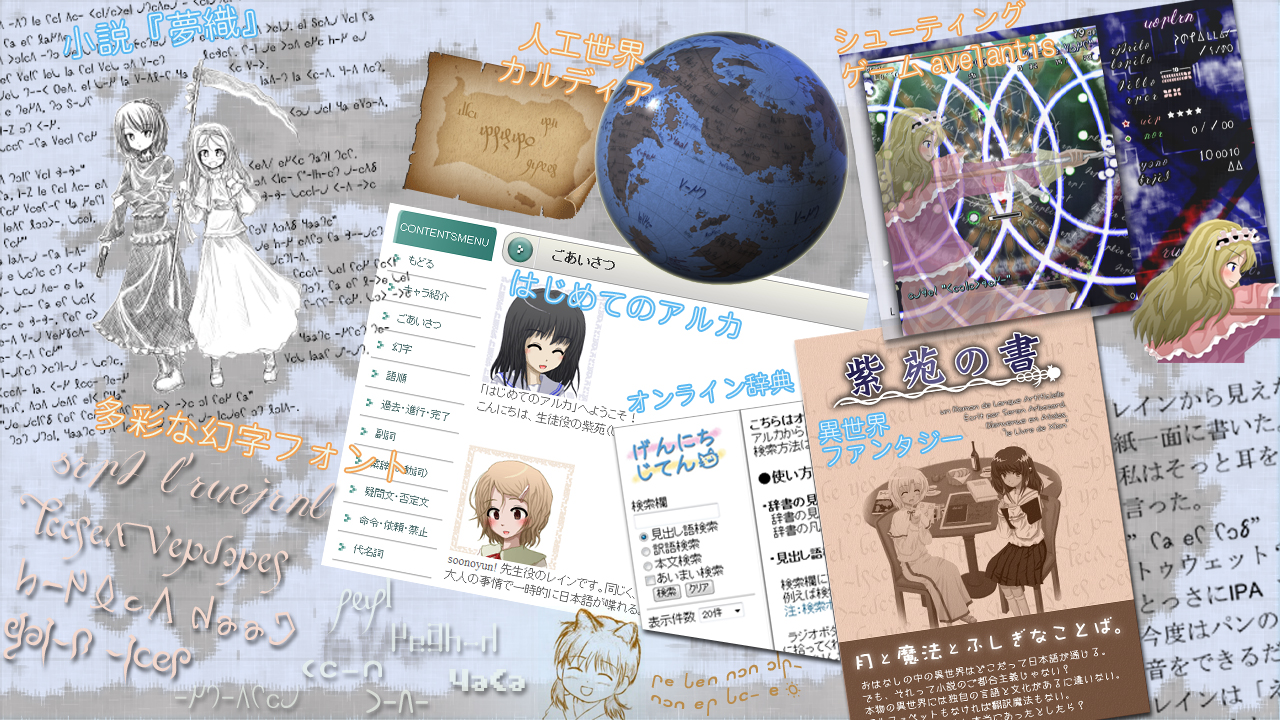
\includegraphics[width=1\textwidth]{ARKA/leis.jpg}
\end{figure}
有余裕的话,还可以看看\href{http://www44.atwiki.jp/conlang_arka/pages/1.html}{ARKA的特性}和
\textattachfile{attachfiles/語法論-人工言語の見えない心臓.pdf}{语法论-人造语言无形的心脏(日语)}
,我们也推荐\href{http://conlinguistics.org/arka/e_study_kit.html}{给初心者的指南}.

\small{
译者的话:

我翻译了初学者课程的第一部分,就是之后章节Lein的课程.但是整个网站的内容太多,我难以完全翻译.
希望有心人可以接续我的愿望.这本书以latex制成,等到网好的时候我会把所有的文档放在github上.
大家都可以来参与翻译.

\quad --亿年-二孤旋
}
\section{相关网页}

%arka维基:\url{https://arka.fandom.com/wiki/ARKA_Wiki}

Arka词典(Arka<->日语):\url{http://mindsc.ape.jp/klel/}

\part{Lein的课程}
\chapter[人物介绍]{人物介绍}
%\chapter[短标题显示在页面]{长标题显示在目录}

% {\small\textit{
% \quad Sors de l'enfance, ami réveille toi!\newline
% \quad \quad —Jean Jacques Rousseau.}
% \footnote{Ekster el infaneco,amiko veku!}
% \\}

% 
% 
\includegraphics{pngs/x_sena.png}
% \label{x_sena}
% 
\begin{minipage}[b]{0.4\linewidth}

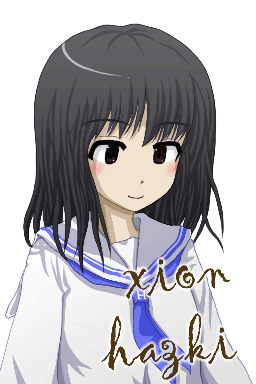
\includegraphics[width=\linewidth]{pngs/aria1.png}

\end{minipage}
\hfill
\begin{minipage}[b]{0.6\linewidth}
17岁的高二学生.

梦想着有一天被召唤进异世界的少女.

被召唤到了Atlas,和Lein一行人相遇,学习Arka.

性格老实内向,在地球朋友很少.%\tiny 

特长是合气道和剑道.喜欢荞麦和胡萝卜.{\textcolor[rgb]{1,0.92,0.92}{普通}}

喜欢的类型是智性的年长男性.为花粉症烦恼.
\end{minipage}





\begin{minipage}[b]{0.4\linewidth}

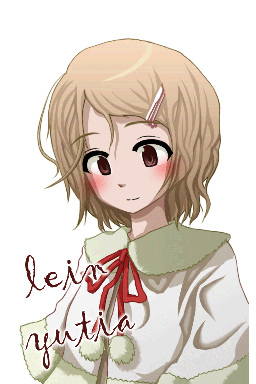
\includegraphics[width=\linewidth]{pngs/aria2.png}

\end{minipage}
\hfill
\begin{minipage}[b]{0.6\linewidth}
16岁前期的Arna大学的学生,在Ridia带的1班

住在中央Arna城的Nermes-Ridia Avenue大街.

救下来了从地球的紫苑,而后开始教她Arka.

性格稳重大方,又单纯。容易害羞,朋友很少。

特长是家务和外语。不擅长运动。喜欢猫。{\textcolor[rgb]{1,0.92,0.92}{平}}

喜欢的类型是像哥哥一样的温柔男性,为自己的幼儿体型苦恼。 

\end{minipage}




\begin{minipage}[b]{0.4\linewidth}


\includegraphics[width=\linewidth]{pngs/aria3.png}

\end{minipage}
\hfill
\begin{minipage}[b]{0.6\linewidth}
17岁前期Arna大学生.在Raldura带的8班.

住在中央Arna市的Poen-Fulmiia街.

和Lein是同级生,是从祖上以来就是占卜师

性格和看起来相反,非常好放.喜欢调戏别人,搞点恶作剧.

特长是预知和预言.画画很菜.酒量大.{\textcolor[rgb]{1,0.92,0.92}{丰满}}

喜欢的类型是小巧可爱的女孩子.因为自己太高了而烦恼.
\end{minipage}

\begin{minipage}[b]{0.4\linewidth}


\includegraphics[width=\linewidth]{pngs/arsen.png}

\end{minipage}
\hfill
\begin{minipage}[b]{0.6\linewidth}
25岁的魔法研究所所员,专攻语言学.

住在中央Arna市的Tiitel-Ridia街.

召唤部的公务员Hain Alteems的儿子.

性和稳重,有绅士风度.在Arna大学还任导师,对学生很和蔼.

特长是Yuvel(Arna的一种武术).直爽,厌恶曲意逢迎.{\textcolor[rgb]{1,0.975,0.975}{你想咋}}

喜欢刚强的孩子.因为父亲太伟大了而烦恼.
\end{minipage}



    
    
    
    
    
    
    
    
    
    
 



\chapter[问候]{问候}
%\chapter[短标题显示在页面]{长标题显示在目录}

% {\small\textit{
% \quad Sors de l'enfance, ami réveille toi!\newline
% \quad \quad —Jean Jacques Rousseau.}
% \footnote{Ekster el infaneco,amiko veku!}
% \\}

\emoji{x_sena}
% \begin{figure}[h]
% 
\includegraphics{pngs/x_sena.png}
% \label{x_sena}
% \end{figure}

欢迎来到Lein的课程!

大家好, 我是学生紫苑. 现在17岁,在上高二.

\emoji{l_sena}

Soonoyun [so:nɔjɯn]! 我叫Lein,是你的老师. 我也是Arbazard中学的学生.
\footnote{这几位女生是``紫苑之书''中的主人公,Nias Avelantis制作了立绘(还包含以后会介绍的Alia和Arshe).感谢他的贡献}

我本来不该说汉语的,但是编辑叫我说我就说吧. :)

\emoji{x_knoos}

那个,你说的第一个词是啥? 额... soonoyun ?

还有Arbazard又是哪?我在世界地图上没找到.

\emoji{l_rana}

Soonoyun 意思是``你好''. 它可以指代早上好,中午好和晚上好.有用吧?
Arbazard是Atolas的一个国家,而Atolas是我居住的星球. 我们国家通行的语言就是Arka.

\emoji{x_naki}

Arka不是地球上的语言吧?怪不得我没见过这些字母.
\begin{figure}[H]
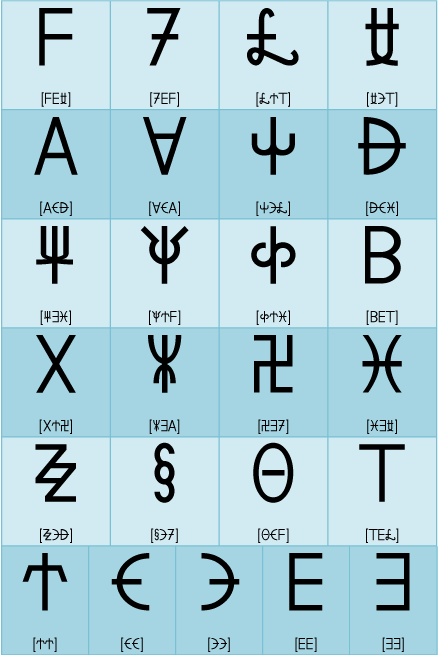
\includegraphics[width=0.5\textwidth]{ARKA/klandi.png}
\end{figure}
\emoji{l_deyu}

这些字母是幻字的大写字母.
20个是辅音,5个是元音,总共有25个.
在Arka中,幻字被叫做hacm.

\emoji{x_lek}

这也忒难记了吧!

我可能记得住E 和 F, but...

\emoji{l_ket}

其实, 我们很少用大写字母,你只要记住这些小写字母就行了.
\begin{figure}[H]
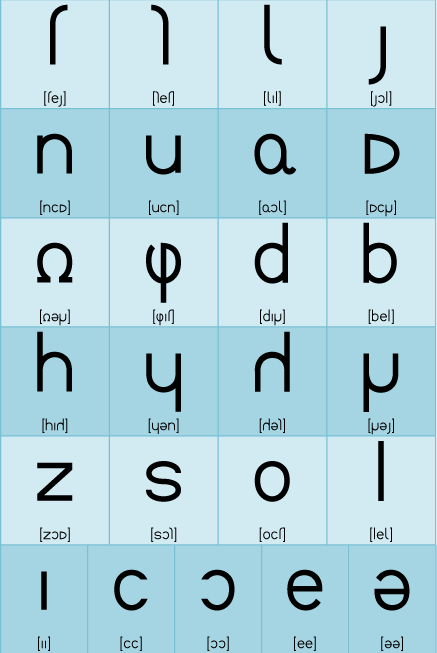
\includegraphics[width=0.5\textwidth]{ARKA/lemal.png}
\end{figure}
\emoji{x_tisse}

这样啊,那说不定能行.所有字母都只有一画,有些字母还和拉丁字母很像.
幻字来自别的世界,但某种程度上还真是相似啊.

\emoji{l_rana}

你发现了奇妙的东西呢.不过关于字母的文章现在对你来说还太难.

\emoji{x_lo}

小写字母虽说简单,但我还是要花点功夫记.现在嘛,我要用拉丁字母转写Arka.
在我熟悉字母表之前,我还是先看这个语言的转写版凑合.
\begin{figure}[H]
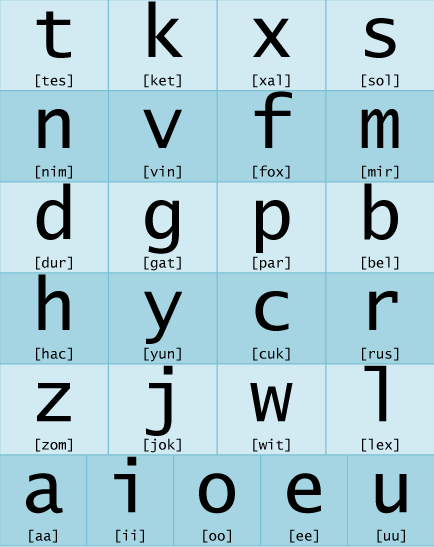
\includegraphics[width=0.5\textwidth]{ARKA/tenxa.png}
\end{figure}
\emoji{x_lo}

转写的Arka大部分都还行.就是``x''和``c''发音有些奇怪.``x''发[ʃ](像``shop''里的``sh''),``c''是卷舌的 R (像西班牙词``burro''里的``rr'').

So, ``c''是齿槽颤音[r], whereas ``r''是齿槽近音[ɹ].

其他的字母...? ``y'' ([j])像"yes."的``y'', ``j'' ([ʒ])像``vision''的``s''.``h''([h])像``happy''里的``h'', ``w'' ([w])像``wise''的``w''.

\emoji{l_rana}

熟悉幻字的时候就用拉丁转写吧. ``tx'' ([tʃ])像  ``church''的``ch'',``ts''发``cats''的``ts''.

幻字是专门书写Arka的,所以用来写Arka就很有效.一步一步来嘛.

很多字母都相互对称;我小时候就经常把``tes''混成``ket''.长大了就分的清了,就像你区分``d''和``b''一样.

\emoji{x_sena}

看来我应该一步一步来,多动笔写写.
不管咋样,我该练练转写啦.\textbf{``x''发``shop''的``sh'', ``c''发西班牙语``burro''的``rr''.}
说干就干!

%"([a-z]+)"
%``$1''



\chapter[幻字]{幻字}
%\chapter[短标题显示在页面]{长标题显示在目录}

% {\small\textit{
% \quad Sors de l'enfance, ami réveille toi!\newline
% \quad \quad —Jean Jacques Rousseau.}
% \footnote{Ekster el infaneco,amiko veku!}
% \\}


\emoji{l_sena}

Soonoyun(你好)! 是我,Lein.今天我们来上第二课吧.
紫苑啊,你记住幻字的拉丁转写了吗?

\emoji{x_asex}

那是.我现在看转写词没啥问题,驾驶碰到"x"和"c"要小心. 
"x"发音像"shop"的"sh","c" 像西班牙语"burro"里的"rr".
把"c"当做[r]有点怪,但是我不想依赖别的例子去记它.
"シ"在Arka中写作"xi",所以我的名字在Arka里写作"Xion",不是"Shion".


\emoji{l_iks}

你别把xion读成ksion了,OK?

\emoji{x_seernik}

Xion... 我想到一个播放器\footnote{Zeon,瑞翁电器} :)

\emoji{l_niit}

先别管讲笑话,现在发音如何了?

\emoji{x_nal}
还是不习惯.但我会尽力去做的
让我试试这样行不行.顺便把字母表写下来.

% \includemedia[label=lettersong,flashvars={source=ARKA/hacm.mp3},
% transparent,
% passcontext %show VPlayer's right-click menu
% ]{}{APlayer.swf}\\
% \mediabutton[
% mediacommand=lettersong:play
% ]{\fbox{发音}}
% \mediabutton[
% mediacommand=lettersong:pause
% ]{\fbox{暂停}}

\begin{figure}[H]
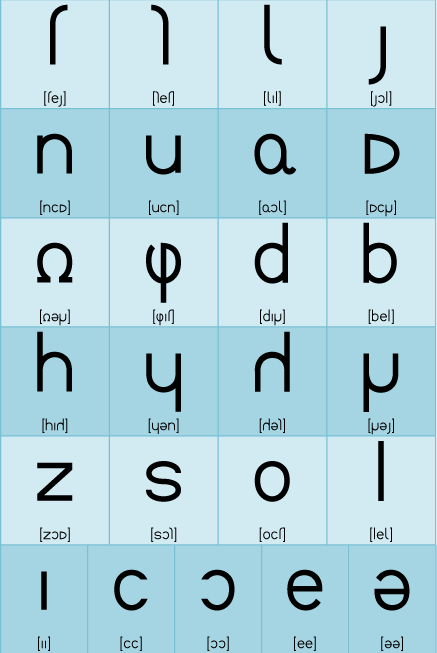
\includegraphics[width=0.5\textwidth]{ARKA/lemal.png}
\end{figure}
Yeah,这就挺不错的(=°ω°)ノニャン♪

"c"就像"burro"里的"rr",但是女生喜欢像日语的"r"一样发音就像"ramen"([ɾaːmen]). 
学术点的讲,就是齿龈闪音.

接下来,来听听\textattachfile{ARKA/hacm.mp3}
{字母歌}吧.
%"([a-z]+)"
%``$1''
\chapter[语序]{语序}
%\chapter[短标题显示在页面]{长标题显示在目录}

% {\small\textit{
% \quad Sors de l'enfance, ami réveille toi!\newline
% \quad \quad —Jean Jacques Rousseau.}
% \footnote{Ekster el infaneco,amiko veku!}
% \\}


\emoji{l_sena_deyu}
今天我们来学习Arka的语序吧!

汉语里,像``黑猫''这样的词,形容词在名词前面,但是在Arka里,你应该说``猫-黑.''


\emoji{x_loki}
你说...像法语那样? ``黑猫''在法语里叫做``chat noir''.形容词``noir''在名词``cat''后面.

在Arka里,就说``ket (猫) ver (黑)'',对吧?

明白了,形容词在名词后面.那么,你们是如何造句子的呢?


\emoji{l_niit}
就像汉语那样.

举个栗子,说``紫苑看到Lein,''你就像``紫苑'' + ``看'' + ``Lein''这样拼起来.你知道的,``主语'' + ``谓语'' + ``宾语.''

``看''在Arka里叫``in'',所以你要说``紫苑看到Lein,''就说:``xion in lein.''


\emoji{x_pil}
这就叫SVO.
在这一点上,Arka和汉语,英语都很像呢.


\emoji{l_deyu}
那么问题来了.
你怎么表达``大狗看小猫''呢?

单词: 大 = kai, 小 = lis, 狗 = oma, 猫 = ket,看 = in


\emoji{x_lo}
形容词在名词后面,so``大狗''就是``oma kai'',``小猫''就是``ket lis.''

语序是SVO,那么...

``Oma kai in ket lis,''这样?


\emoji{l_uni}
好!

嘿呀,你会用Arka造句子了.(v\^{}-°)

OK今天结束之前,我们再来看一个问题.

``给''在Arka里是``fit'',苹果是``miik''.So,``Lein给紫苑一个苹果''应该怎么表达?


\emoji{x_fron}
Arka是主-动-宾,就是``lein fit miik.''

慢着,``给紫苑''怎么说?


\emoji{l_niit}
我们用``a''指示目的方.
``A xion''就是``给紫苑''.合起来说就行了.


\emoji{x_tisse}
``A xion''就像英语短语一样,``to Shion''.``A''就像个介词.
所以答案是``lein fit miik a xion,''吗?
这句子还挺长的.我一开始对Arka一无所知,但现在我已经能说出一个句子了.这种不可思议的感觉...
Lein你怎么表达``看了''或者``给了''?


\emoji{l_sena}
我下次就教你Arka的时态. Doova ([doːva] (下次见)) !

%"([a-z]+)"
%``$1''



\chapter[时态]{时态}
%\chapter[短标题显示在页面]{长标题显示在目录}

% {\small\textit{
% \quad Sors de l'enfance, ami réveille toi!\newline
% \quad \quad —Jean Jacques Rousseau.}
% \footnote{Ekster el infaneco,amiko veku!}
% \\}

\begin{figure}[H]
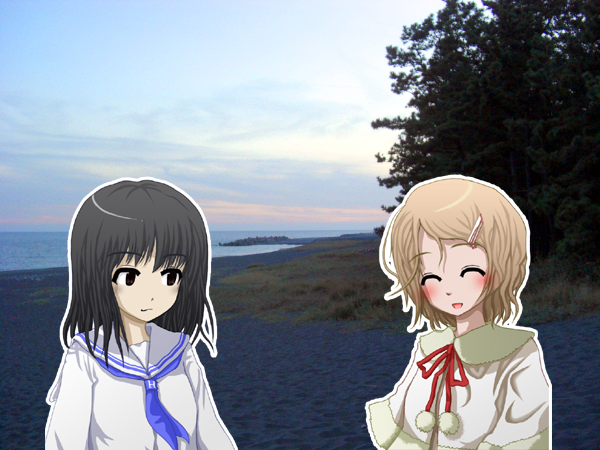
\includegraphics[width=1\textwidth]{ARKA/tier2.jpg}
\end{figure}

Lein: ``我们来海边啦!好-大-的-海-啊!嘿,紫苑,你在干什么?''

紫苑: ``唔...你的腿好细啊.如果我是你的话...''

Lein: ``额...''

紫苑: ``诶~''xion in lein``哦.上次我们学了''紫苑看到了lein.``你也说Arka是SVO型语言''

Lein: ``对对对,形容词在名词后面,记得挺牢的.''


\emoji{x_knoos}
那么,你怎么说``紫苑看到了Lein?''


\emoji{l_sena}
过去时啊,在汉语里,在动词后面加上``了'',在Arka则是``-at''.


\emoji{x_lo}
So,我试着想,``紫苑看到了Lein''就是``xion inat lein,''.

Arka 没有``saw''之类要特殊记的变化,这倒挺简单.没有啥例外吧?


\emoji{l_lo}
我想想...哦哦,动词结尾是元音的话,就不是加``at''而是``-t''.

``Xa''是``在某处'',结尾是元音,所以加 ``-t''.``Xat''就是 ``曾经在某处.''


\emoji{x_loki}
避免元音冲突?

还有``-at''同类型的词缀吗?


\emoji{l_niit}
要表示进行的体
\footnote{译者注:英语原文用的是aspect,日语原文用的是``過去形'',``進行形'',``完了形'',
既然日语原文没有明确是时态(tense)还是体态(aspect),暂且以英语原文为准,说这个词缀表示动词的体态.}
的话,
就在动词后面加``-or''.Axt``是''写``, ''axtor``就是 ''正在写."

如果动词以元音结尾就不加``-or'',而是``-r.'' ,``Ena''是``哭'',那么``enar''就是``正在哭.''


\emoji{x_asex}
在进行体的表述上,Arka和汉语真是不一样.

``-Or''表示进行体.我觉得你下次该说完成体了.


\emoji{l_diina}
猜对了!完成体是在动词后面加``-ik''.

``Axtik''是``已经写了.''

要是动词以元音结尾,就只用加后缀``-k.''


\emoji{x_niit}
``-At''是过去时.``-Or''是进行体.``-ik''是完成体.

等会,将来的事件怎么办?


\emoji{l_uni}
我们不用后缀来表示将来时.

下次我再说吧

\begin{figure}[H]
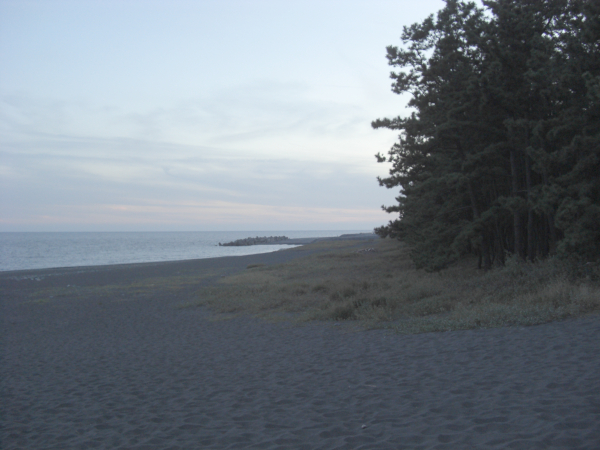
\includegraphics[width=1\textwidth]{ARKA/tier.jpg}
\end{figure}

\emoji{x_knoos}
顺便问一下,Lein,我们现在看的是那片海啊?


\emoji{l_iks}
阿这,我们,在,在,在首都Arna南边,边,边的,的Kateej...(´·ω·`)


\emoji{x_pilp}
其实就是静冈县 :-7


\emoji{l_vexl}
诶呀,这是善意的谎言啦\~{}


%``([a-z]+)''
%``$1''



\chapter[副词]{副词}
%\chapter[短标题显示在页面]{长标题显示在目录}

\emoji{l_deyu} 
\hypertarget{chapter-adverb}{我们}上次学习了Arka的时态和体态,紫苑,你还记得吗?


\emoji{x_vesn} 
动词加``-at''变成过去时.对应的,``-or''变成进行形,``-ik''变成完成形.

``写''是``axt,''那么``axtat''就是``已经写了,''而``axtor''意思是``正在写'',``axtik''意思是``写完了.''

英语的进行时和完成时还要加``be''或者``have''之类的,但Arka里面加后缀就行了.

那未来怎么表达呢?像``将要写.''


\emoji{l_niit} 
你应该在动词前面加一个副词, ``sil.''

``Axt sil''意思是``将要写.''跟``-at''不一样,``sil''不是后缀,所以不要写成``axtsil,''而应该写``axt sil.''


\emoji{x_niit} 
``Axtat'' (写过了)比``axt sil'' (将要写)要短呢.

这是为什么呢?


\emoji{l_sena_deyu} 
好问题!因为过去时出现得更加频繁.

过去时,进行时,和完成时比较短是因为它们出现的更频繁.不常出现的时态就用``sil''之类的副词表达.

这些是Arka的其他副词.我把常用的副词打成表:
\begin{table}[h!]

    %\caption{常用副词}
    \begin{tabular}{|c|c|c|} % {l|c|r}<-- Alignments: 1st column left, 2nd middle and 3rd right, with vertical lines in between
      \hline
	  \textbf{词汇} & \textbf{简要翻译} & \textbf{意义}\\
      \hline
      lax&  想要做&  希望\\\hline
  	van&  要做&  意志\\\hline
  	sen&  能&  可能性\\\hline
  	vil&  不能&  没有可能性\\\hline
  	das&  为什么不&  提议\\\hline
  	fal&  必须&  义务\\\hline
  	flen&  可以&  许可\\\hline
 	xiit&  让我们&  劝诱\\\hline
  	yu&  被&  被动\\\hline
    \end{tabular}

\end{table}    

\emoji{x_asex} 
Arka的副词相当便利呢.像英语之类的,助动词先得一堆.

当你表达``想要'',只需要加上``lax'',``为什么不''只要用``das''时,那可舒服了.

另说一下,这些都能是动词吗.我是说,一般的动词都像``高高地''或者``猛烈地'',这样.


\emoji{l_sena} 
``强,猛''是 ``vien'',``猛烈地''是 ``vienel.''要把形容词变成动词,你只需要加``-el''后缀就行了.

Arka有两种副词,一种想辅助词一样的,和形容词加``-el''转化来的.

结尾是元音的,就不加``-el'',而是加``-l''.``aalo''意思是 ``灵巧,''那么``灵巧地''就是``aalol,''而不是``aaloel.''

来个小练习,``紫苑可以写Arka''要怎么说?
%dexterous:灵巧

\emoji{x_lo} 
``xion axt sen arka''?


\emoji{l_ket} 
嗯~,对了!♪


\emoji{x_knoos} 
嘿, 我在表里找到了``被动语态''呢.这是啥?


\emoji{l_diina} 
``yu''产生被动语态. ``xion axt arka''意思是``紫苑写Arka,''这是主动语态.

要把它变成被动语态,就--\\
\textbf{
\quad1) 在动词后面加``yu'': xion axt yu arka\\
\quad2) 把主语和宾语倒过来: arka axt yu xion}

--就这样.

``arka axt yu xion''意思是``Arka被紫苑写.''


\emoji{x_loki} 
OK,Arka不用加``be,''我也费不上记动词的过去分词.只要加``yu'',然后被主宾关系倒过来就行了.

我逐渐地能写复杂的句子了呢.

但是我还不能翻译``这是一个苹果.''
Lein老师,你下次会教我Arka的系动词吧(\FiveStar ω\FiveStar)


%``([a-z]+)''
%``$1''



\chapter[系动词]{系动词}
%\chapter[短标题显示在页面]{长标题显示在目录}

  

\emoji{x_sena} 
呐, Lein,这是啥?

\begin{figure}[H]

\includegraphics[width=0.7\textwidth]{ARKA/ket.jpg}
\end{figure}

\emoji{l_ket} 
猫!

喵喵\~{}.

我之前给你说,猫在Arka里叫做``ket''.

``这是猫'',就说``tu et ket.''


\emoji{x_niit} 
Arka里注释在最前面呢,所以``tu''就是``这个,'' ``et''意思是``是.''


\emoji{l_asex_kal} 
对,``et''是系词.``tu et oma''意思是``这是一只狗.''


\emoji{x_lo} 
``oma''的地方可以填形容词吗?


\emoji{l_sena_deyu} 
可以.``tu et kai''意思是``它很大.''


\emoji{x_loki} 
变过去式就加``-at'',对吧?

那么``它之前很大''就是``tu etat kai''吗?


\emoji{l_pels} 
不是的,应该说``tu at kai.''

系词出现得相当频繁,所以我们不说``at''而是说``etat.''

这对``or''(进行时)和``ik''(完成时)也适用.

``tu or kai''意思是``它正在长大,''而``tu ik kai''意思是``这已经长大了.''


\emoji{x_tisse} 
哈哈,这样我也不用记``was''或者``been''这类的分词了.

Arka的系动词就是``et.'' ``tu et miik''意思是``这是一个苹果.''

句子的顺序就和``xion axt arka'' (紫苑写Arka)一样呢.记得住记得住.

顺带一说,``紫苑不写Arka''和``紫苑写Arka吗?''应该怎么说?


\emoji{l_nax} 
你是说疑问句和否定句吗?

OK,我下次就教你.



%``([a-z]+)''
%``$1''



\chapter[疑问句,否定句]{疑问句,否定句}
%\chapter[短标题显示在页面]{长标题显示在目录}

  



\emoji{l_diina}
这是我前几天在公园散步时看见的花.

紫苑,这是樱花吗?
\begin{figure}[H]
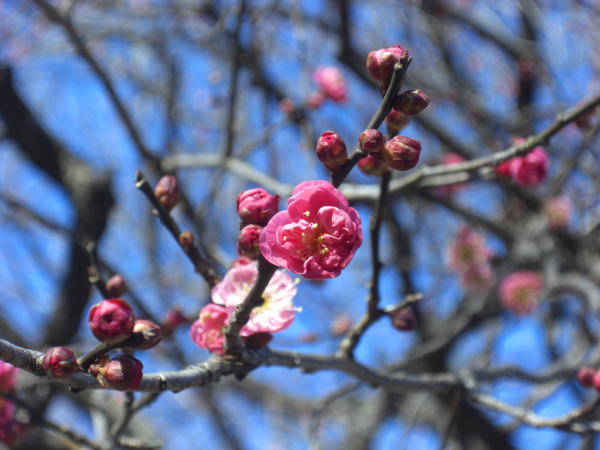
\includegraphics[width=0.7\textwidth]{ARKA/ping.jpg}
\end{figure}

\emoji{x_lo}
额,这是梅花,不是樱花哟

呐,在Arka里怎么说"这是梅花."?

\emoji{l_asex_kal}
"这是梅花"应该说"tu et ping"。"tu et"就是上次讲过的

"这是樱花"也差不多,说"tu et seron"。

"这是樱花吗"就在句子最后加上mia."tu et seron mia?"

不过很多场合我们不特意加"mia",只是在句子后面加一个问号.


\emoji{x_pil}
疑问的时候语调要上扬一些呢.
相比于英语的"Do you...?"Arka要简单呢。跟汉语在句末加"吗"比较像.


\emoji{l_sena}
另一方面,"这不是樱花"应该说"tu de seron".
de一个词就表示系动词的否定,像是"isn't"一样.
顺便一说,女生不用"de",而用"te".


\emoji{x_niit}
那么我其实应该说"tu te seron"吗.

%ともあれ、「~でない」はdeね。「~DEない」と覚えようw ------翻译不过来的梗
另外,"不写"应该怎么说呢?


\emoji{l_xanxa}
be动词以外嘛,就在动词前面放副词"en".

axt是"写"、那么"en axt"就是"不写".


\emoji{x_demo}
哦......"紫苑不写Arka"就是"xion en axt arka"吧。

让我总结一下:

\textbf{
疑问句:只是在句尾加"mia"\\
否定句:be换成de,另外就是在动词前面加"en".
}

\emoji{l_deyu}
最后来做个小测试吧.

试着写下"这是猫吗?","这不是猫,是狗.","紫苑会写Arka吗?"这三个句子
答案就在下回的开头.atte!(加油!)




%``([a-z]+)''
%``$1''



\chapter[祈使句]{祈使句}
%\chapter[短标题显示在页面]{长标题显示在目录}

 
\emoji{l_asex_kal} 
我们上次学了Arka的疑问句和否定句
紫苑,你把作业做的咋样了?


\emoji{x_pels} 
"它是猫吗?"; tu et ket mia?

"它不是猫,它是狗"; tu de ket. tu et oma.

"紫苑不写Arka吗?"; xion en axt arka mia?

--对吧?


\emoji{l_ket} 
OK,好样的!

最后一个句子是疑问句和否定句的组合,看起来你也做得不错呢.


\emoji{x_fron} 
副词"en,"后面接上动词表示否定.在英语里,类似的词"not,"出现在动词后面.

Arka里形容词在动词后面,但是"en"却在动词前面.这有点奇怪.

还有其他在动词前面的词吗?


\emoji{l_asex_kal} 
有,我接下来教你Arka的祈使句.

你要表示祈使,就在动词前面放"re"."re lef"意思是"跑!"

我给你把出现在动词前面的词列成表
\begin{table}
    \begin{tabular}{|c|c|c|} % {l|c|r}<-- Alignments: 1st column left, 2nd middle and 3rd right, with vertical lines in between
      \hline
	  \textbf{词汇} & \textbf{简要翻译} & \textbf{意义}\\
      \hline
      re&  做&  命令\\\hline
  mir&  请做&  要求\\\hline
  den&  不准&  禁止\\\hline
  fon&  请不要&  劝阻\\\hline
    \end{tabular}
\end{table}

\emoji{x_lo} 
"请不要写"是"fon axt."

你怎么说"请不要走"或者"请过来"?


\emoji{l_deyu} 
"fon ke"和"mir luna."

"ke"是"走,"然后"luna"意思是"来."


\emoji{x_asex} 
明白了.

这意味着祈使句可以向英语和汉语一样省略主语.

"you come here"也可以是"come here."


\emoji{l_sena} 
这个省略不必强求.

"ti mir luna"就像"你过来一下."


\emoji{x_tisse} 
在Arka里"You"是"ti"吗?

说到"你," 我还没有在Arka里学到"我","他"之类的代词呢.


\emoji{l_iks} 
唔...

\emoji{x_knoos} 
嗯?


\emoji{l_hik} 
其实我一直在......故意避免它们......


\emoji{x_knoos} 
为啥?


\emoji{l_reiv} 
因为真的很烦......(´·ω·`)





%``([a-z]+)''
%``$1''



\chapter[代词]{代词}

%\chapter[短标题显示在页面]{长标题显示在目录}

\emoji{l_diina} 
\hypertarget{chapter-pronouns}{来},我来教你Arka的代词,像``我'',``你'',``他'',``它''.


\emoji{x_seernik} 
你上次不是说它很复杂吗?先拣主要的说吧.

首先,无生命物的代词是什么?我是说, ``这个,'' ``那个'' and ``他.''


\emoji{l_asex_kal} 
``这个''是``tu,''``那个''是``le.''

我们没有``它.''


\emoji{x_lo} 
OK, ``tu''和``le.''啊,你之前教过我``tu.''
那像``我''这样有生命物的代词呢?


\emoji{l_niit} 
``我''是``an'', ``你''是``ti.''

``他''和``她''都是``lu.'' ``lu et xion''意思是``她是紫苑.''

``lu''意指这个人离说话人近,而``la''意指这个人离说话人远.


\emoji{x_loki} 
那就是说``lu''是``这个人,''而``la''是``那个人.''

``她/他''是一样的,但是``lu''和``la''却有区分.

与``tu''和``le''的区别就在于有生命.

还行吧,现在Arka大代词还没什么奇怪的地方.

\emoji{x_tisse} 
哦哦,明白了.有``I,'' ``my,'' ``me'' and ``mine''\footnote{此处为英语原文的例子,日语原文是「私が」「私の」「私を」「私のもの」}
等等的区别,就像英语和德语那样,对吧?


\emoji{l_deyu} 
不不不,Arka只有``我''和``我的''.
``Me''和``I''都是``an,''而``my''和``mine''都是``ant.''
代词的种类只有两种:``我'' 和 ``我的,'' ``你'' 和 ``你的,'' ``他\\她'' 和 ``他\\她的.''我给你列个表:
\begin{table}[H]
    \begin{tabular}{|c|c|c|c|} % {l|c|r}<-- Alignments: 1st column left, 2nd middle and 3rd right, with vertical lines in between
    \hline
	我&  an&  我的&  ant\\\hline
	你&  ti&  你的&  tiil\\\hline
  	他/她(近)&  lu&  他/她(近)的&  luut\\\hline
	他/她(远)&  la&  他/她(远)的&  laat\\\hline
	这个&  tu&  这个的&  tuul\\\hline
	那个&  le&  那个的&  leet\\\hline
	\end{tabular}
\end{table}

\emoji{x_pil} 
右边的看起来都以``l''或者``t''结尾.

也许他们确实不规则,不过总比英语的``I,'' ``my,'' ``me'', ``mine''要好些.其实也不难.


\emoji{l_iks} 
我刚才列出的代词是最普通的.

我给你说过,女生用否定系动词的时候不用``de''而是用``te''.

Arka的代词用法有很多种.明确谁在说,谁在听,作用很大.
根据说话者的不同,代词也有不同.你看下面这个表,女生倾向于用这些代词.
\begin{table}[H]
    \begin{tabular}{|c|c|c|c|} % {l|c|r}<-- Alignments: 1st column left, 2nd middle and 3rd right, with vertical lines in between
    \hline
	我&  \textcolor{pink}{non}&  我的&  \textcolor{pink}{noan}\\\hline
	你&  \textcolor{pink}{tyu}&  你的&  \textcolor{pink}{tuan}\\\hline
  	他/ 她(近)&  lu&  他/ 她(近)的&  luut\\\hline
	他/ 她(远)&  la&  他/ 她(远)的&  laat\\\hline
	这个&  tu&  这个的&  tuul\\\hline
	那个&  le&  那个的&  leet\\\hline
	\end{tabular}
\end{table}

\emoji{x_loki} 
这样啊.人与人之间用的代词确实不一样呢
但是仔细一看,只有``我,'' ``我的,'' ``你''和``你的''有变化呢.


\emoji{l_hik} 
像你这样的女生喜欢自称``non,''但是其他类型的会叫``yuna''或者``noel.''

男生也用好多代词,甚至中性的人类和有灵魂的非生命体也有自己的代词.总共有\textcolor{pink}{12}种代词.

另外,Arkaz最大的挫折就在\hyperlink{appendix-pronouns}{这个代词表}......


\emoji{x_nik} 
?Σ(°ロ°;)

每个人和每个人的代词都不一样...! 但是在区别说话者的个性时非常有用.


\emoji{l_pels} 
每个代词都有复数形式,``我们''是``ans,''``我们的''是``antes''.

当然,这些复数形式也因人而异.性格内向的萌妹子会用``lena'' (我们)和``lenan'' (我们的).


\emoji{x_iks} 
OK,我,服了.这,就,是,代,词.(;\CircleShadow ω \CircleShadow )ゞ


\emoji{l_diina} 
确实是.不过你平时只要记住``an行''和``non行''就行了.不用全记住的.

不过,你刚才也说了,多亏了这些多彩的代词,Arka可以鲜明地表示人物性格.


\emoji{x_asex} 
辞藻华丽呢.


%``([a-z]+)''
%``$1''



\chapter[格词]{格词(前置词)}
%\chapter[短标题显示在页面]{长标题显示在目录}

\emoji{l_xanxa} 
好,我们之前搞定了难受的代词,现在来学习Arka的格词\footnote{英语为 Preposition (一般称介词),不过她还特地造了一个词 caser.}吧.


\emoji{x_nau} 
Lein老师,格词是什么呀?


\emoji{l_niit} 
这是Arka的一个术语,就像英语里的介词一样.

举个例子,``to''是``a,''而``from''是``i.''


\emoji{x_asex} 
我们已经学了介词``a.''
``Lein给紫苑一个苹果''就是``lein fit miik a xion.''
``a'' indicates a destination, a recipient and so on.


\emoji{l_asex_kal} 
Yeah.英语里介词数量很小,但是Arka的介词,规模可是,相当宏大.


\emoji{x_knoos} 
二十几个?


\emoji{l_txu} 
额...100个以上...(汗)


\emoji{x_lek} 
我缓一会\quad w.


\emoji{l_myulla} 
嘛,其实常用的格词也就是十多个.

再说,大多数格词其实是和名词差不多的东西.

``hal''是``在上方,''但是也可以作名词.


\emoji{x_pil} 
是这呀,你不早说,吓死我了.

英语里``Front''是个名词,但``in front of''是介词短语.但对于Arka,它们的形式都是``sa.''你不需要单独记它.


\emoji{l_xakl} 
说回来,有这么多介词有啥好处呢?


\emoji{x_fron} 
唔?

我想想... 唔...想不来.


\emoji{l_diina} 
反过来想.

像英语那样前置词太少,不就产生了各种问题嘛.


\emoji{x_lo} 
要是没有很多介词,就要把一个介词赋予多重意义.事实上,``on''和``in''就有一大堆意思.

英语学习者就经常纠结什么时候该用什么介词.


\emoji{l_niit} 
相反,感谢这丰富的数量,Arka的学习者就清楚地知道哪里用什么介词.

确实你要记``frem''(附近)or ``fol''(...期间)之类一大堆介词,但它们仅仅是普通的形容词和介词,费不了多少功夫.
我把常用介词列成表:
\begin{table}[H]
    \begin{tabular}{|c|c|} % {l|c|r}<-- Alignments: 1st column left, 2nd middle and 3rd right, with vertical lines in between
    \hline
	a&  	为,到 \\\hline
  	i&  	从 \\\hline
  	kon&  	使用 \\\hline
 	ok&  	和...一起 \\\hline
	ka&  	在(地点) \\\hline
	im&  	在(时间) \\\hline
	man&  	因为 \\\hline
	ol&  	如果 \\\hline
	\end{tabular}
\end{table}

  
    

\emoji{x_loki} 
``man''(因为)和``ol''(如果)在Arka里不是连词而是介词吗?

``Shion和Lein一起写Arka''就是``xion axt arka ok lein''?


\emoji{l_uni} 
bingo!

别把``ok''说成``kon''啊,我可不是笔啊.



%``([a-z]+)''
%``$1''



\chapter[关系词]{关系词}
%\chapter[短标题显示在页面]{长标题显示在目录}

\emoji{x_niit} 
嘿 Lein,我们现在学了很多语法了,还有多少?


\emoji{l_deyu} 
语法的话这就是最后一节了.

这节是关于关系代词的.


\emoji{x_lo} 
我学英语的关系代词是总是非常懵.

我们看这一个句子 "I know a girl who is cute."
如果先行词不是"girl"而是"book"的话,"who"就会变成"which."
在"I know a girl whom he likes"里又是"whom",因为这里的女生是宾语.


\emoji{l_asex_kal} 
对啊

准确的来说,Arka并没有关系代词."Who","which"和"whom"在Arka里都是"le",但"le"是连词.

试着把"I know a girl who likes cats"翻译成Arka?

Arka和English有一样的句子结构,所以我就给你一点提示.

know = ser

a girl = fian

likes = siina


\emoji{x_demo} 

哦,有点难啊.

句子结构是一样的,"who"在Arka是"le",so--
"an ser fian le siina ket"?


\emoji{l_ket} 
干得漂亮!

那么,"I know a girl whom he likes"又如何呢?


\emoji{x_pels} 
"He"是"lu"或"la."我们现在用"lu".

用"who"还是"whom"都可以,因为Arka只有"le"--
"an ser fian le lu siina,"对吧?


\emoji{l_asex_kal} 
Yeah.即使是"book"而不是"girl",你也可以用"le".我是说Arka不区分"who"或"which."

另外, 如果"le lu siina"变成了"le alis siina,"你就应该说"l'alis siina."


\emoji{x_lo} 
在原有开头的词前面,"le"就变成了"l".


\emoji{l_diina} 
对, 对.

你以后就能用"le"造复杂的句子,所以习惯就好.


\emoji{x_nal} 
OK,这样语法就告一段落了吧.


\emoji{l_niit} 
上了我这么长的课程你已经累了吧.

我们下次就远离语法了.


%``([a-z]+)''
%``$1''



\chapter[语调]{语调}
\emoji{l_asex_kal}
既然讲完了语法,今天我带了朋友来哦.

\emoji{a_nax}
soonon♪
听说紫苑在学Arka,就过来玩了哦\~{}


\emoji{x_nau}
啊,这不是占卜师Alia嘛,欢迎欢迎.

\emoji{x_nik}
诶,等会!

为什么你也在说汉语啊( ゚Д゚)


\emoji{a_reps}
啊哈,我一切皆有可能哦。占卜师什么都能看见哟.

你看,拿着这个水晶,不管是考试的答案,还是彩票的中奖号码(呼呼呼...


\emoji{x_seernik}
诶呀诶呀,这已经超过占卜师的领域了吧 w

\emoji{x_dagd2}
我记着《紫苑の书》的一个优点是就是排除了这种投机取巧吧?

别老整这胡来胡来的好吧.我作为主人公可不能坐视不理啊.


\emoji{a_niit}
haan, xom xenon xook fan al axel kokko arka hot, nee lein, nonno?

(OK,我们现在全篇用Arka交流吧,呐,lein?)

saa, noel jins vil toal iskan rok sarlots t'inar atu e(axte

(不知道有多少读者会点右上小红叉w)


\emoji{x_vexl}
――别别别这么我求你了!!(゚ロ゚;)


\emoji{l_sena}

好好好.

昭和漫才还是打住吧,今天是关于语调的。


\emoji{x_lek}
额!!Σ(°Д°;


\emoji{l_asex_kal}
你觉得「Arbazard」哪里重读比较好呢?

其实arbazard在哪里重读都可以.


\emoji{x_lo}
这就是说不用记单词重读的位置?比英语简单啊。

但是,因为不知道哪里可以放重音,反而更迷惑了吧.

有什么决定方法么?


\emoji{l_diina}
每个方言都有自己的放重音的方式。
Arbazard有3个方言,我和Alia说的北方方言和日语重音相近.


\emoji{a_rans}
嘛,虽说是日语,但也有各种各样的方言。

这里说的是东京方言的外来语口音。


\emoji{x_niit}
原来如此。那么“Arbazard”在Lein和Alia的发音中“za”的部分也很强吗?


\emoji{l_niit}
对就像读片假名一样\footnote{意思就是有些是开头重音,有些是开头低,中间高,后面再低(主要是在复合词中的后一个词下去).}

其实重音放错了也没事,不必在意.


\emoji{a_niit}
重音法则虽然有,但很难,这里就不讨论了。

法则也有例外,不过,后面介绍的词典里有“重音”的标签,所以没关系。

\chapter{数字}
地球虽然有很多种语言,但数字大概哪里都是阿拉伯数字呢。

Arbazard毕竟是异世界,没有阿拉伯数字吧?


\emoji{l_naki} 
没有呢……阿拉伯数字。
不过作为替代,有这样的数字呢
(0~9まで)
\begin{figure}[H]

\includegraphics[width=0.7\textwidth]{ARKA/alx.jpg}
\end{figure}

\FiveStar 读法

0:yuu

1:ko 

2:ta 

3:vi 

4:val 

5:lin 

6:kis 

7:nol 

8:ten 

9:los 

\emoji{x_naki} 
0和1以外,一点看不懂(-ω-)


\emoji{a_reps} 
不过,因为是十进制的计数法,所以比较容易计数吧
顺带一说,4,5,6和7,8,9的末尾是规则的l,n,s,这可以方便记忆呢。


\emoji{l_niit} 

数数的方法和日语一样呢.10读作on.

13是on和vi的拼接,onvi。

20是ta和on的拼接,taon。


\emoji{x_knoos} 
百和千之类怎么说?


\emoji{l_asex_kal} 
百是gal,千是kot,万是sen。

例如24,345,就读做tasen valkot vigal valon lin。


\emoji{a_niit} 
和日语不同的是,一万不是kosen,就是一个sen,这个要注意
\footnote{日语里面如果是"一千"和"一百",就能省略"一",只说"千"或"百",这一点对"万"不适用.但是Arka是可以的}.


\emoji{x_niit} 
原来如此。

那么,"4个女孩子"怎么说?


\emoji{l_sena} 
是val fian。

Arka没有"人"啊"个"啊这样的量词\footnote{原文为"助数詞",译者暂时没有在网页中找到"两筐篮球"之类关于"量"的描述./*TODO*/},
只要把数放在名词前面就可以了。

顺带一说,fian val这样在名词后面九上数字也可以,这种用法,就表示序数,"第4个女孩子"


\emoji{x_sena} 
霍霍,这么方便啊.

只要换个地方就能变成号码。
\chapter{接续词,纯词}
\emoji{l_xanxa} 
现在,「初Arka 1」就剩下两章了呢.

最后作为赠品处理连词和死生动词.这次是连词.


\emoji{x_niit} 
接续词是说and和or之类的?


\emoji{l_asex_kal} 
对对,"and"读"o".

我们在字典的语源栏往往用"/"代替"o".

xion/lein就是"紫苑和Lein".


\emoji{a_rans} 
另一方面, "或"是"az."
"miik az lisik"意思是"苹果或橘子."


\emoji{x_knoos} 
这样啊."与"和"或"在Arka是接续词.

不过,"但是"和"然后"在Arka也是接续词吧?


\emoji{l_asex} 
"但是"和"然后"是纯词,不是接续词哦.

"但是"是tal、"然后"是yan或see.它们都是纯词,现在就记住比较好.

所以你怎么说"紫苑来了,但是Lein没来"?


\emoji{x_lo} 
嗯..."来"是luna.

过去式是动词加上-at,lunaat…….


\emoji{a_niit} 
可惜啊.luna以元音结尾,不是加"-at",而是加"-t".


\emoji{x_nakx} 
哦啊,我把这个忘了(\^{}-\^{}. 是lunat啊.
然后否定形是动词前面加en:en lunat.所以说――
"xion lunat. tal lein en lunat",这样?


\emoji{l_uni} 
对哒!好棒!
\chapter{死生动词\&后记}
\emoji{l_sena_deyu} 
这就是Lein课程1的最后一节了.

今天我来教你死生动词.\footnote{英语原文是switching verb,说这对动词就像开关一样.}


\emoji{x_seernik} 
好可怕的名字!


\emoji{l_nakx} 
哎嘿嘿(\^{}-\^{};
生动词"ar"意思是"激活某物,"死动词"is"是"关闭某物."
就像汉语里的"开灯"和"关灯"一样

在Arka,"ar"和"is"这对动词的职责要大一些:"ar ata"是"开会\footnote{汉语里就没有"关会"这种说法,而是单独有"散会","闭幕"之类的动词.},
"而"ar pam"就是"开灯."


\emoji{x_tisse} 
看起来非常有用呢.
"ar +设备"就是"激活设备." "ar + 事件"就是"举行事件."

\emoji{a_rans} 
yeah.所以我们叫"ar"生动词.

"is ata"意思是"结束会议,"而"is pam"就是"关灯." "is"就叫做死动词.

你不需要记很多搭配,只要用"ar"和"is"就能表达很多复杂的句子.


\emoji{x_pilp} 
明白了

所以"alia ar lein"......


\emoji{l_vexl} 
我可不是道具!(>\_{}<)


\emoji{x_naki} 
抱歉啦 :)


\emoji{a_pilp} 
(Lein说是道具的话还真是方便......全自动做饭洗衣机w)

    
\emoji{x_nal} 
这样Arka讲座的理论编就告一段落了吧?

二位也辛苦了.多亏你们的教导,我现在对Arka掌握了许多。



\emoji{l_nax} 
你也累了吧,紫苑.

也感谢各位读者们 :)

理论编到此结束\~{}\~{}

我下次在Lein课2会给你讲一个Arka爱好者画的漫画,无论如何都来一下哦\~{}
\chapter{如何使用字典}
    

\emoji{l_nax} 
大家好,我是Lein.

我在初Arka1里面已经讲了Arka的语法.

不过我觉得大家会想"我虽然学习了语法,但是仍然不会读Arka."

紫苑,你呢?


\emoji{x_niit} 
确实,我知道Arka是SVO,形容词在名词后面,但是仍然不会读.

\emoji{l_sena} 
所以,我们在Lein课2里面就教大家如何通过依旧学了的语法阅读Arka.(*°---°)


\emoji{x_nakx} 
说真的,背单词太难了.

确实Arka的语法比英语简单,但是怎么也逃不掉背单词啊.


\emoji{l_ket} 
碰到不会的词就查Arka的在线字典好了.

你不用在电脑上安装什么.并且信息总是更新的,靠得住. 


\emoji{a_nax} 
这是一个电子词典,比纸质的词典更方便.

只要查的次数足够多,那么不用费力记单词也能记住.

首先,你可以查\href{http://conlinguistics.org/klel/}{Diaklel},Arka的在线词典.

\emoji{x_sena} 
Arka的词典被叫做"幻日词典"呢,"幻"是指Arka么.\footnote{英语原文称"Lunar Dictionary"}

在左上的检索栏输入么?


\emoji{l_sena_deyu} 
用普通的键盘就行了.

你也可以按拉丁字母序查找单词,而不用Arka的字母序.


\emoji{x_demo} 

搜索结果按字母序列出.

我以为它会像Arka字母序一样列出来呢,像 t, k, x, s...


\emoji{l_sena} 

Arbazard的字典里,单词以Arka字母序排列.

不过在Diaklel,有一段时间单词是以Arka字母序排列的,但是对用户不友好所以在08年就停止了.


\emoji{a_lo} 

Diaklel在2005年以Arka字母序编写,但学习者用起来非常困难.

不过现在非常趁手就是了.


\emoji{x_lo} 
Hmmm.另外,它由17000多个词.对于人造语言来说真的很大.

我的名字也在里面吗?哦,字典里没有"xion".因为我是地球的女生么?


\emoji{a_naki} 
不一定.也许你应该查一下你的全名,"xion hazki".

或者点一下"模糊检索(あいまい検索)"?

模糊检索会找出任何包含"xion"的词或短语.


\emoji{x_lo} 
这样啊

诶,我找到了.

说"她是紫苑之书的女主角,一名日本的高中生,故事从她的十七岁生日开始. 恶魔Meltia将她召唤到Atolas.
在这里她见到了另一位女主角Lein,,和男主角Arsye.她和恶魔之杖Varde战斗,拯救了Arbazard."

看起来字典总结了书中的内容呢.


\emoji{l_diina} 
Diaklel不只是字典,更是一本百科全书,对文化也有好多的记载.
关于文化的记录都写在[culture]一栏.查查看.


\emoji{x_knoos} 
Lein,苹果在Arka叫什么? 我想通过"苹果\footnote{其实要用日语词"リンゴ".}"这个词查Arka的对应词.

难道这个字典如果不知道Arka词就不能用了么?


\emoji{l_deyu} 
可以用.把"标题栏检索(見出し語検索)"换成"译语检索(訳語検索)."

你现在就能把它当成日-Arka词典来用.

去掉"模糊检索"然后把"リンゴ"写到搜索栏里.按回车或者查询键.


\emoji{x_niit} 
找到了,Arka里苹果是miit.

你在"译语检索"里也能用"模糊检索"吗?

    
\emoji{a_niit} 

可以.

你也可以查"青苹果(青りんご)."里面的"苹果".


\emoji{x_nau} 
哦,太好了(°∀°)

这个字典确实有很低功能呢.


\emoji{l_uni} 
\href{http://conlinguistics.org/arka/study_yulf_140.html}{字典的巧妙使用方法}中还有很多其他的诀窍,请读一读
那么下次使用aav一项,说明本文所讲的用法。
\chapter{阅读字典条目}
   
\emoji{l_sena} 
soonoyun, 这是实践编的第二课。我们来学习通过Diakel来轻松地理解Arka。

我们马上来翻开词典,检索"aav"吧.

----

[名词]锁, chain 

[动词] 将yul用锁拴住 

%[letters] link 
[メタファー(隐喻)] 链接,联系

rd;raavyu,lsl.xik 

13:raavyu (锁) 从古Arka 

raabyu:raavyu:la kolett (线,绳) 

[文化] 普通金属制.项链是身旁的锁.锁也用于禁止进入. 

[成语] yun aav 顺藤摸瓜 

[用例]

aav oma a nial 用锁拴住狗

gil at aav soven la tianal. 那两个人的恋爱关系是靠钱。

diretan fosat yu yun aav 顺藤摸瓜把犯人抓起来了。

----


\emoji{x_lo} 
这里.[名词]和[动词]是词的类型吧?

"aav"意思是"锁",作动词时也是 "把...锁起来".

那么"[隐喻] 链接"是什么?


\emoji{l_diina} 
姆...因为你是我的朋友,我才在这里.

你我的链接就是友谊,这里"aav"就象征它.

一般,词语的意思从最基本(最常用)到最引申(最罕见)排列.

所以作为"链接"的意思在这个表里排得靠后.


\emoji{x_pil} 
词典很方便呢.

那接下来两行"rd;raavyu,lsl.xik"和"13:raavyu (锁)从古Arka"是啥?


\emoji{l_sena} 
这是词源学的部分.

你可以看到此什么时候,怎么样产生的.


\emoji{a_sena} 
这个太难了,我下次再给你讲.

接下来这一行, "raabyu:raavyu:kolett,"是关于外国词语的.

他们是"fiilia-filveeyu," "lyudia-arbazard"和"siizia-lutia."


\emoji{l_nakx} 
不过我保证你也不认识它们.

前面的两个是作为Arka基础的两门古语.然后Lutia的语言对Arbazard的语言有很大影响.

"锁"在Arka叫"aav",但是在Lutia叫"kolett".你也许有一天会用到它.


\emoji{x_demo} 
我明白了.接下来的这一行是[文化].这读起来有意思.
然后是"成语"和"例子".


\emoji{a_sm} 
有时候[语法]栏比[文化]来得更早.

通过读[语法],你能明白这个词是怎么用的.就像名词范围和词语搭配这些.


\emoji{x_loki} 
嗯... 语源和外语部分是[语法],[文化]等等的分界线呢.

词典结构清晰,很好读.并且句子短,换行也多,对眼睛很友好.

谢谢你,我明白怎么阅读词典了.我下次来翻译一下Arka句子.
\section{通过漫画理解}

\emoji{l_sena} 
大家好.

习惯阅读幻日辞典的方法了么?

今天我们来借助字典读真正的Arka文本吧.


\emoji{x_sena} 
哇哦。真是实践编的感觉呢σ(°ー\^{}*)

so,要解读什么?虽然掌握了语法,也会使用词典,但是那种特别难的小说还是......

不过,教科书一样的例文却没什么意思...。


\emoji{l_nax} 
所以今天就来这个吧。
\begin{figure}[H]
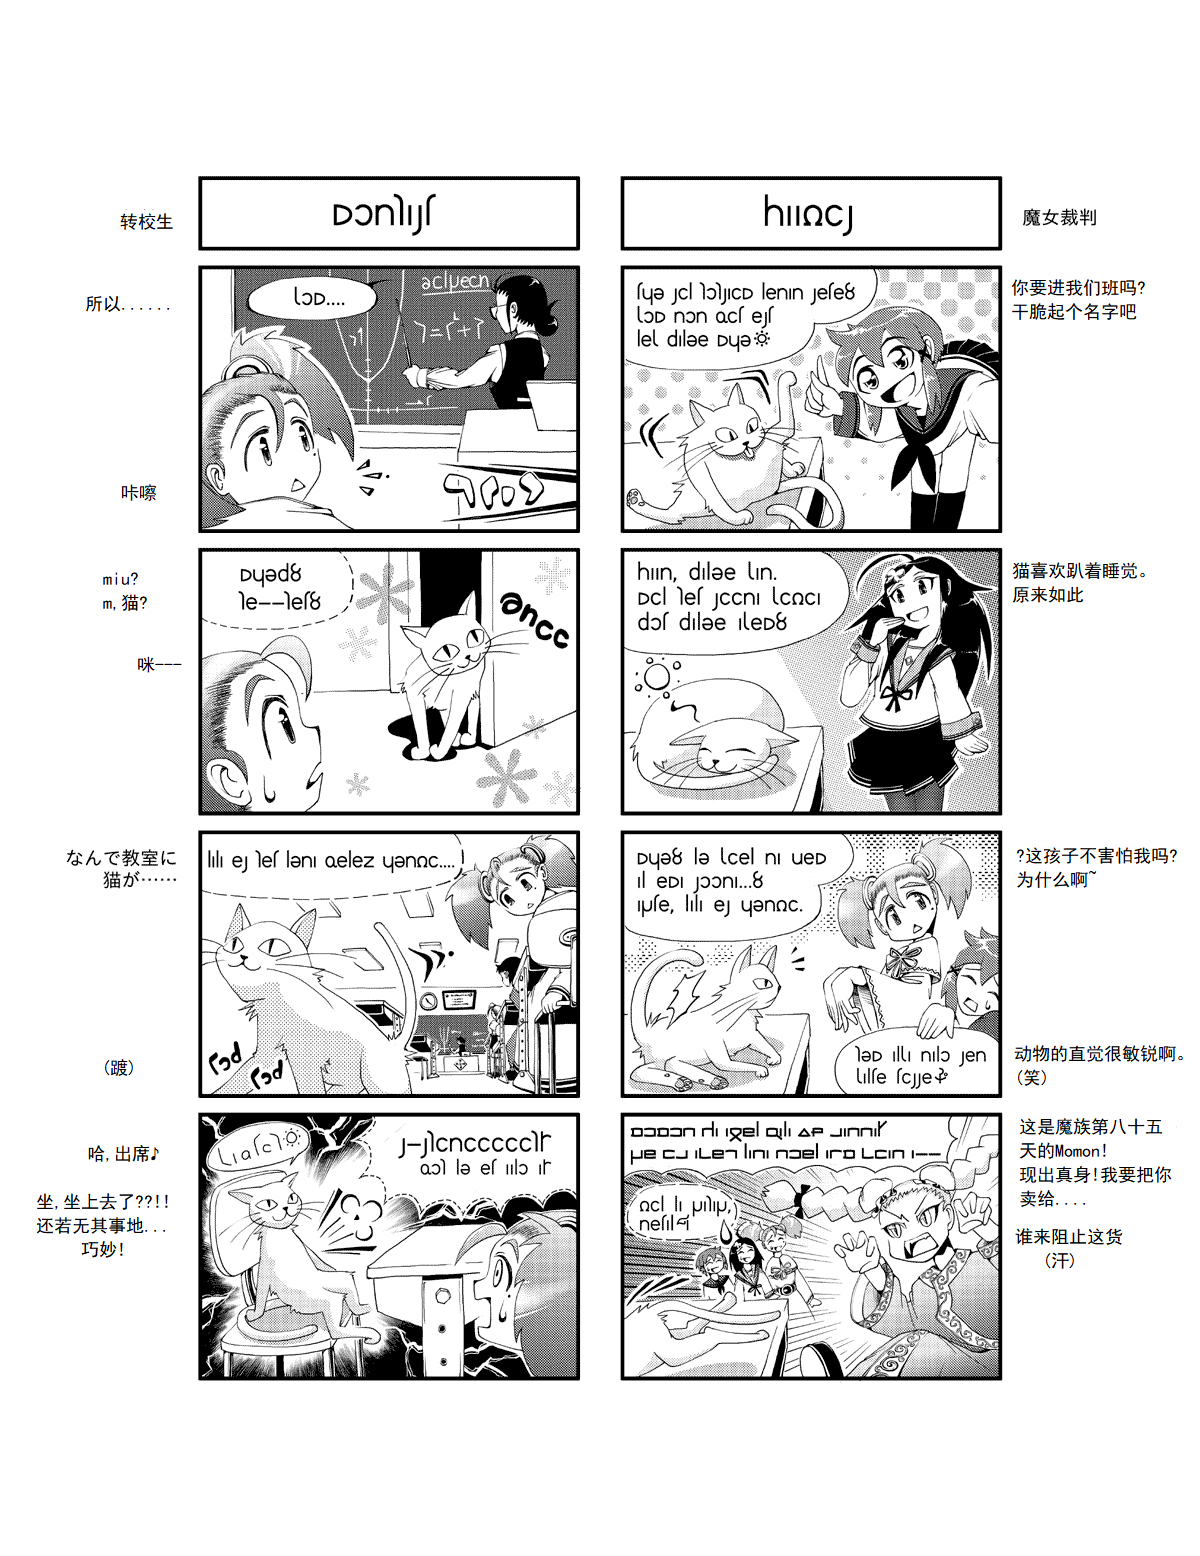
\includegraphics[width=\textwidth]{pngs/xarl2.png}%或者height=\textheight
\end{figure}



\emoji{x_nau} 
啊,是四格漫画呀,也有异世界呢♪


\emoji{l_rana} 
%これは「中央アルナ大学」に通う4人の女の子のお話よ。<a href="works_xale_1.html" 「ねこにっき」って言うの。
4和漫画用起承转合的结构叙述,容易理解.从画面里也能看到文化和举止,意外地有学习性呢.

今天我们用右边的漫画,一格一格地读.

\emoji{a_nax} 
顺便说一下Arna大学就是我和Lein上的学校哦.

说是大学,对日本人来说也只是高中生吧.

lein在Lydia带的1班,我在Lardura带的八班.不知道这几个人在哪一班.


\emoji{l_ket} 
我觉得是猫班♪

\chapter{第一格(前)}

\emoji{l_ket} 
《猫的日记》是由"悠闲的xia","大姐姐一样的mifa","稳重的yure","孩子气的feer"四个人登场的欢乐向漫画.

虽然都是Arna的大学的学生,但是由于和日本的学年制度不同,3个人都只有15岁.

今天学校来了一只白猫.

进入了Xia的教室、一边闲逛一边坐上了没有人的桌子.

这是到了休息时间,xia他们跟猫说话的场景。


●1格
\begin{figure}[H]

\includegraphics[width=0.5\textwidth]{ARKA/uni1.png}%或者height=\textheight
\end{figure}



\emoji{l_diina} 
这个棕毛就是"悠闲的xia".

她是从首都Arna南边的Kadish搬过来的,那是滨海的都市,是温暖的度假胜地。

Kadish人多是成熟悠闲的类型,xia也是。


\emoji{x_tisse} 
穿着日本的水手服呢.Arbazard也有这样的衣服吗?

看图同时了解文化可是一石二鸟啊.

这样说...哇,没有转写的幻字啊ーヽ(;´·ω·)ノ生幻字啊{\tiny 怕怕}

\footnote{作者注:严格来Arna大学没有制服,为了分辨角色而做了权宜.}

\emoji{l_nakx} 
先从字母转写开始吧.慢慢来.

我也算做了一些转写练习,记得可牢了。

\FiveStar 转写

xia: tyu sil koksaim lenan sete? xom non fit est lex palue myu (xante


\emoji{x_loki} 
嘿,那个数字8一样的东西是问号啊.

最后的文字是啥?工厂的地图记号吗,还是太阳....


\emoji{l_deyu} 
太阳吗?嘟嘟---.这是月亮哦,满月。

表示说话者的语调非常高兴。

满月在Arka叫xante,转写的时候就写"(xante"吧.


\emoji{x_nal} 
连表示说话方式的文字都有呢。好厉害。日语的(笑)啊,"♪"啊之类的。

不过,最初的句子是"tyu sil koksaim lenan sete?"吗。果然到正篇了吗,单词一下子就难起来了。

......咦?好像tyu和sil在理论编教过了。tyu是女用词"你",sil是表示未来形的副词。

啊啊,记忆模糊了(>\_<)。在词典查sil吧。

----

[名词]未来、将来

[纯副词]\~{}将要做.未来时的副词。

[动词]\~{}将要做。未来时的系词。

[形容词]未来的

[反意词]ses

19:制:sikt(之后)

【用例】

amir sil 未来的丈夫


----

\emoji{a_niit} 
表示未来形的副词就是sil。是纯副词方面的呢。

另外还有"未来的名词含义呢"。同时掌握不同类型的语义,感到知识增加了。

不过,"tyu sil koksaim lenan sete?"的sil视作哪一种词类比较好呢?


\emoji{x_niit} 
额......tyu不是动词,那么sil作副词的解釈就说不通了。

既然Arka是SVO,tyu应该是主语.这样sil就是动词,这是3号的语义。

呐,Lein,未来时的系词又是什么?不是,我知道未来时,只是......


\emoji{l_rana} 
系词就是be动词哟。

sil一个词就是will be的意思。


\emoji{x_lo} 
这样啊。所以意思就是"你将是\~{}"吧。

......有什么用呢,tyu sil koksaim lenan......。

啊,要是看仔细些,lenan也在理论编出来过呢。%<a href="study_mive1_10.html" 

那么.意思就成了,"你将是我们的koksaim"。


\emoji{a_pels} 
さすがにkoksaimは引かないと分からないわね。
参考までに。

\emoji{x_niit} 
同样的班......啊,就是说同班同学啊。

就是说"你将是我们的同班同学"。


\emoji{a_tia} 
这就对了!

那么问题来了。koksaim的哪个部分是"同"哪个部分是"班"呢?


\emoji{x_pels} 

等会等会......等式是koksan,同一个小组的伙伴是koksems......kok还是koks呢......。


\emoji{a_niit} 
很好的着眼点呢。那么,"同"就是"kok"。

比较上下的单词,就能加深理解,这就是词典的好处呢。


\emoji{x_lo} 
怎么说呢,这个字典连物理,地理,气象的用于都有呢......。

还有,"tyu sil koksaim lenan sete?"最后的"sete"是什么啊?

----

[文末纯词][rente]kok
古

----


\emoji{x_naki} 
啊呀,满是tag......。

诶,这是啥?


\emoji{l_asex_kal}

这个啊,"sete可归类为句末使用的纯词","sete是稳中女子所使用的词语","意义与kok相同"。

文末纯词就是日语的``\~{}ね''``\~{}さ''``\~{}だよ''``\~{}だわ''``\~{}でしょ?''这样的单词。

而后,有时间的时候、去调查一下yunk和milia吧。

先不管了,这时候应该查查kok――

----

[形容词]同じの

[反意词]koot

[格词]和\~{}相同、像\~{}一样

[文末纯词]"\~{}么?"请求确认。
[接续词]t和k都是同一类\~{}。

[数学]合同\footnote{几何变换中就有合同变换,指变换后的图形在与原图在大小和结构上都相等.}

[音乐]simile\footnote{指照前面方式演奏}

13 古:koko。纯词用法有``和我的想法相同吗?''这样的意思。

【成句】im kok 同时
【用例】

ti siina miik kok? 你喜欢苹果么?

an kok ti et kai. 我像你一样大。


----

\emoji{x_vesn} 
啊、找到"文末纯词"了。

嘿、像``\~{}么?''一样有确认的意思呢.

这么说、"tyu sil koksaim lenan sete?"是``你就是我们的同班同学么?''的意思吧。

哦这样啊。进入教室的猫住习惯了,是说的这个意思。

呼哇ーー,好不容易才弄明白了。


\emoji{l_niit} 
辛苦啦♪


\emoji{x_nal} 
谢谢ー。

好厉害的完成感啊,Lein!

好!好一部分先休息,我们来攻略第二格吧!
\chapter{第一格(后)}

\emoji{x_asex}

好,到第一格的后半了.然后是"xom non fit est lex palue myu(xante"。

non是"我",fit是"给".理论编还记得住。

non在意义上应该是主语,不过,为什么主语前面先来了一个xom?

xom,xom......

----

[格词][文首纯词]"所以"、较弱的因果关系

19:较弱的son

----

\emoji{x_knoos} 

弱化版的son啊,那son又是什么?

----

[格词][文首纯词]既然、因此、中等結果意味

古:从so派生

[语法]

"因为"的对应。表示结果。


----


\emoji{x_lo} 
"既然"......啊。有"じゃあ"一样的感觉啊。

[文首纯词]这样标注,就像日语的接续词一样呢.

啊,这样啊。所以放在主语non前面。

xom non fit就是"那么我给你"的意思吧。

不过,给的东西......是哪个?


\emoji{l_hik} 

(我、放置play......(T\_{}T)


\emoji{x_loki} 
est是名字吗。给猫一个名字,哦.

然后是lex palue......?

呐,Alia,查lex出现了两个东西.

----

lex

[格词]给的对象,和yul值同一格。
%~と

[反意词]xel

15:恣意

lex(2)

[语言]l的文字

14:制:知識

[语法]

第20个幻字。最后的辅音字母。



----

\emoji{a_sm} 

既然lex(2)是字母的名字,这就是上面的那个。

yul指的是目的语哦。在这里指est(名字)就是目的语。

既然写了X lex Y,就有X = Y的意思。


\emoji{x_tisse} 
总之、est lex palue就理解成est = palue吗。

换句话说,"名字=palue"...啊,猫给猫起的名字就叫"palue"啊。


\emoji{l_ket} 

乒乓!\footnote{译注:奇奇怪怪的拟声词}

并且palue是"向阳处"的意思.暖洋洋的喵。

最后的myu啊――

----

[感動词][文末纯词]myu?,myun

19:新生词从古myup逆成
\footnote{日语词的形成法之一,
本来不是词尾的部分,由于形式上类似而被看作词尾,从而形成新词的现象。
由「たそがれ」形成「たそがる」,由double形成「ダブる」之类。}。

[语法]

猫风的文末纯词。表示心里愉悦平和


----

\emoji{x_pil} 

这也是文末纯词吗。看起来文末纯词可以在句子结尾表达说话者的心理呢。

sete是确认、myu是平和。

温和......我,我方了.


\emoji{a_niit} 

对于我们Arbazard人,语言是用来------

1:组织道理、

2:分析感情

――的工具哦。在内观和主张上都有特化.


\emoji{l_rana} 

这样一说,能细致地分析整理自己的感情,在Arbazard长大真是太好了。

连表示这些的专门形容词都有。

----

naxiris

[形容词][积极]心思纤细,可以感到机微.

[反意词]alnaxiris

20:na/ixirius(心之镜)

[语法]

用多种样式准确地表达自己的感情.
相对地,像对不论什么东西只是说"烦",就是alnaxiris。
naxiris有知性和风流的形象,具有积极色彩。
繊細而易伤,神经质等意味则不用这个词.在"知道细微的变化"这个意义上使用。
alnaxiris则有贬义。


----

\emoji{x_sena} 
这种形容词都有!?外语的学习变得有意思了啊。

总之、"xom non fit est lex palue myu (xante"的翻译就是"那么我就叫你洋洋\footnote{原文为ひだまり,照着起了类似的名字}吧♪"

呼------、总觉得漫画的第一格就累死了\~{}。


\emoji{l_niit} 
不论谁一开始都是这样哦。

不过从我看来,你学习的其实很惊人呢.

到此就休息吧,辛苦了.












\chapter{第二格}
\begin{figure}[H]

\includegraphics[width=0.5\textwidth]{ARKA/uni2.png}%或者height=\textheight
\end{figure}



\emoji{l_sena} 
那个黑发女生就是``稳重的yuule.''

她是从远方的Lutia来的.

人们说Lutia人都非常聪明,并且她,yuule尤其聪明,简直是天才.

不过有些冒失,xia她们经常调戏她.和feel关系不错.


\emoji{x_niit} 
看起来既聪明又听话.

还有冒失,嗯,是我了. 你看,把手搭在嘴边,感觉就很清爽.


\emoji{l_niit} 
嗯,除去稳重和清爽确实很像.


\emoji{x_jo} 
......

OK,我们来转写字母吧.

\FiveStar 转写

yuule: haan, palue xan. mil ket siina xidia pot palue axem?


\emoji{a_sm} 
有一些在第一格里就有了.


\emoji{x_pil} 
确实,读起来比前面更简单了.

``haan''是个感叹词,意思是``我明白了.''

还有``xan...''

我要找哪个?

----

xan

[名词]真,真实,真相

[形容词]真

[文首纯词]其实

[副词]真的,确实

[同义词]yuliet

[反义词]enx

13:制Arka:古Arka:xin (真) < xan (真实存在) < xal (存在)

xan(2)
[rente]xa
18:ridia

----

\emoji{l_sena} 
你找的是``xan(2).''

女生倾向于说``xan'',而不是``xa.''

``xa''在这.

----

xa

[动词]sol 在 yul (地点)存在

[文末纯词]注意到

[副词]状态动词的初始态

古Arka:xal

[语法]

xa (前缀): xagart (收费) 
mi (前缀): migart (免费) 

----

\emoji{x_loki} 
``xa''出现在句尾,所以是文末纯词,意思是``注意.''

这种想法就像日语的``あ、そうだ。今日は雑誌の発売日だった'',最后的``タ''\footnote{想想``哦,今天是发售日呀!''里面的``呀''}一样.

或者说,像``あぁ、あそこに見えるのは富士山か''中的``か''之类。
 

\emoji{a_reps} 
就是就是.

当发现了之前不知道的事情时就可以用``xa''.

    
\emoji{x_asex} 
所以,``haan, palue xan.''意思就是``我明白了,它的名字是洋洋.''

那就是说, yuule 明白了xia在第一格给猫起的名字.

\emoji{x_knoos} 
嘿,那个动词的``xa''呢, what does ``sol 在 yul (地点)存在''又是啥?


\emoji{l_sena_deyu} 
``sol''是主语,``yul'' 是宾语.``yul''在这时候就指地点.

如果你是主语,你在学校里,那就说``xion xa felka'',意思是``紫苑在学校.''


\emoji{x_loki} 
明白了,词典里还写了动词主语和宾语的类型.


\emoji{a_ku} 
那我顺便就教你动词搭配吧.关于什么样的名词和动词搭配.

``xa''的搭配,是``sol (人/物)在 yul (地点).''

每个动词都有自己的搭配:``lat (放入)''的搭配是``sol (人) 使 yul (人/物) 进入 a (地点).''

----

lat

[动词]sol (人) 使 yul (人/物) 进入 a (地点)

[名词]入口

[动词]收拾 > fitl

[动词]进入学校或公司 > lod

[antonym]rik

13:制Arka:古Arka:luta (出)

【成句】

hino yul sa lat 差一点就/到极限了

lat, toot, zok, rik 起承转合。入口、坡道、顶上、出口:比喻山路。

【用例】
an hinot ena sa lat. 努力忍住眼泪。

an hinot jo sa lat. 差点就爆发了。
----

\emoji{x_niit} 
你看下动词搭配,就知道该用哪些词了.


\emoji{l_diina} 
下一句是``mil ket siina xidia pot palue axem?''.

我给你解释下``mil''字典说它表示较弱的推断.

``因为''是``man'',这在Lein课1里面讲过了.但是 ``mil''也是 ``因为.''


\emoji{x_knoos} 
那他俩有什么区别呢?


\emoji{l_deyu} 
``man''表示原因和结果的距离近. ``mil''则表示原因较弱,我的意思是,不稳定.

女生倾向用``mil'',少用``man'',这是为了舒缓语气.


\emoji{x_asex} 
OK, ``mil'' 表示 ``因为'',句子是 ``mil ket siina xidia pot palue axem?.''

``ket''是主语``猫'',``siina''是动词``喜欢.''

``xidia''是 ``梦.'' 那么句子的意思是 ``猫喜欢梦.''?


\emoji{l_reia} 
不是,``xidia''也是动词.句子里有两个动词.

``xidia''确实是 ``梦,''不过这里只表示 ``睡觉'' ,这是女生的委婉哦.本来``睡觉''是``mok''.


\emoji{x_loki} 
所以这个句子的意思是``Cats like to sleep.''

那 ``pot''又是什么意思?

----

pot

[名词]内部

[格词]在...里面

[反义词]tant

古Arka:pot, poto

----

\emoji{x_lo} 
``pot''是一个介词,意思是``in.''

``pot palue''意思是 ``在palue里面.''

不过,palue不是那只猫的名字吗. ``他喜欢睡在他里面''?!


\emoji{a_naki} 
啊,不不,不是, ``pot palue'' 里面的palue是个名词,表示``有太阳的地方.''

他的名字也表示``有太阳的地方''.


\emoji{x_asex} 
现在我明白了.

``mil ket siina xidia pot palue axem?''意思是``猫喜欢睡在有太阳的地方,所以你叫它洋洋,对吧?''

yuule这是在确认她的想法.


\emoji{l_ket} 
对.

你已经到漫画的折返点了. atte! (加油!)












\part{语言学上的Arka}
\chapter[Arka与其他的人造语言有什么不同]{Arka与其他的人造语言有什么不同}

\subsubsection{1:拥有先验的人造语言}

新生的Arka是以古Arka和制Arka为基础而形成的。
这些都是先验的。简单来说,就是不抄袭英语等自然语言的意思。
但是,完全排他性地排斥自然语言并实现先验是在中后期Arka以后。

\subsubsection{2:拥有先验的人工文化}

Arka拥有独特的文化设定。
avom(狼)是军队和士兵的象征,比起凶猛、残忍的负面形象,更具有勇猛、果敢的形象。
这是没有文化设定的语言无法决定的。没有文化设定就无法定义狼的形象。
即使没有文化,也可以定义狼作为生物物种的名字,但不能设定象征和形象。

\subsubsection{3:具有先验的人工风土}

Arka拥有独特的人工风土Atlas。Atlas相当于虚构的地球。
主要使用Arka的国家阿尔巴莎德相当于地球上所说的南法。
因为小麦是主食,所以pof(面包)和koka(切片)等作为单纯词分化出来。相反,大米和稻子是同一个单词past。
如果没有风土设定,就无法定义如何划分世界。

另外,文化Antis和风土Atlas相加的就是人工世界卡勒底亚。

把人工语言Arka和人工世界Kaldia加在一起,就叫做幻奏。

语言、文化、风土都是先验的,而且做到这种程度的只有幻奏

语言、文化、风土都是先验的,而且被塑造到这种程度的,除了幻奏以外别无他法。(2010年)

另外,实际上在网络和现实中使用的先验语言这一点也非常有特点。(同年)

(一般来说,后验式人造语言更容易应用。先验的实用难度很高)

世界语等,是有名的后验语,所谓的模仿自然语言的语言。
与先验比较,后验语不费功夫,所以马上就能做出来。

\subsubsection{总结}

正如多次重复先验的那样,独创性和创造性是Arka的特点。

原创词汇、独特的虚构文化等,把重点放在编织“不依赖任何东西的纯粹的空想世界”上。特别强调艺术要素。
\chapter[Arka在人造语言学上的意义]{Arka在人造语言学上的意义}
语言、文化、风土都是原创的。并且详细地创造了这些。
这种组合是人类史上的首次尝试,在学术和艺术上都具有深远的意义。

古Arka有自然语言的流入,制Arka是机械的,不能说是人类的语言。也就是准备不够。
新生的Arka纯粹是“虚构的自然语言的创造”,在学问和艺术上的意义在于尝试创造到何种程度。

这是最脱离国际辅助语的方针。世界语的情况下,要考虑如何普及。
语言的普及是一种社会活动,与语言活动是两码事。与世界语不同,阿卡的作者的专业是语言学,比起社会活动,他对语言活动更感兴趣。
Arka的作者不愿随意推广Arka也是因为这个原因。
现行的人工语言的世界是以世界语为中心的国际辅助语的舞台。

世界语是价值观的尺度,甚至是范式。价值观偏向于国际辅助语。
Arka的存在提出了新的价值观。从这个意义上讲,Arka在人工语言史上具有意义。
\chapter[认知语言学层面的Arka]{认知语言学层面的Arka}
%\chapter[短标题显示在页面]{长标题显示在目录}
%Arka的\hypertarget{appendix-pronouns}{位相}

\section{客观把握与主观把握}
在认知语言学中,认知主体可以定义为对事态的把握.认知的模式可以分为两大类.

一种是从事态的外部把握事态的样式,相当于池上(2002,2005)
\footnote{池上嘉彦(2004)「言語における〈主观性〉と〈主观性〉の言語的指標 (1)」『认知言語学論考』No.3 pp1-49 ひつじ書房
――(2005)「言語における〈主观性〉と〈主观性〉の言語的指標 (2)」『认知言語学論考』No.4 pp1-60 ひつじ書房}所说的客观把握.

一种是从事态内部把握事态的方式,同样相当于主观把握.

事实上同一概念,语言学家用各自的术语来表示.
例如,Langacker(1985)将客观把握称为最佳视点阵列(optimal viewing arrangement),中村(2004)设为D模式.
同样是主观把握,Langacker用自我中心的视点排列(egocentric viewing arrangement),中村用I模式.
本文以最容易从字面理解意思为由,模仿池上的术语.

在语言学上并不矛盾的人工语言的制作方法中,``做"型语言(する语言)相当于客观的把握,"成为''型语言(なる语言)相当于主观的把握.
前文中所涉及的特征数量很少,如做·成为,物·事、have·be等,主要是用``做"和"成为''的对比来说明的.
但是,由于本文所涉及的特征数量太多,所以用する语言、なる语言反而会变得晦涩难懂.因此,从这里开始,要把术语统一为客观把握和主观把握.

当然,各个术语的意思各不相同.
例如中村(2004p40)将I - mode称为``西田的认识论'',将D - mode称为``笛卡尔的认识论'',从哲学角度进行了分析.
在这个意义上,术语的语感各不相同,本文为了方便,统一使用池上的术语.

\section{Arka掌握事态的方法}

在前面的文章中,我们已经明确Arka具有客观把握和主观把握两方面的特征.
森山(2009)提出:一般来说,语言的认知主体进行客观把握,很少夹杂主观把握.

将外界事态语言化有``客观把握''和``主观把握''两种把握方法,根据语言的不同,选择哪一种优先,左右着每种语言所具有的整体类型论特征.
但客观把握和主观把握不是规律,而是倾向,所以即使是客观把握型语言也有可能具有主观把握型的语言的特征.Arka就是一个例子.
那么,Arka具体在多大程度上混合了客观把握和主观把握呢?为此,首先要把客观把握型语言所具有的诸特征和主观把握型语言的诸特征,都列出来.
以中村(2004p41)为基础,分析了Arka的各种特征,如下表所示.
与中村(2004)、河原(2009)相比条目数有所增减,
第一行也不是I - mode、D - mode,而是采用了统一的主观把握、客观把握等,适当地进行了编辑.

如果Arka那一列是``客观'',就意味着对这一行的项目要有客观的把握.
反之,如果是``主观'',就是主观把握.
在客观>主观的情况下,可以主观把握,但表示客观更自然,主观>客观则相反.
根据列的不同,也有特殊表示,在验证栏特别记录.
\begin{table}[H]
	\centering		 
\resizebox{\textwidth}{!}{
\begin{tabular}{|c|c|c|c|} % {l|c|r}<-- Alignments: 1st column left, 2nd middle and 3rd right, with vertical lines in between
	\hline
	相同的项目&			主观把握&		客观把握&	Arka\\\hline 
	动词的理解方法&		「なる」型语言&	「する」型语言&	客观>主观\\\hline
	认知主体存在的方法&	感受者(有情者)(sentient)&	动作主(agent)&	客观>主观\\\hline 
	状况的理解方法&		「事件」「场所」型语言&	「物体」型语言&	客观\\\hline
	存在和所有&			BE语言&	HAVE语言&	客观\\\hline 
	动词的焦点&			行为中心&	结果中心&	客观>主观\\\hline 
	终结指向&			无&	有&	客观>主观\\\hline
	名词的理解方法&		无界性(unboundedness)&	有界性(boundedness)&	客观>主观\\\hline 
	名词图式&			连续体图式&	个体图式&	客观>主观\\\hline 
	第第一人称代词&		多样&	一定&	主观>客观\\\hline
	敬语&				不发达的文法范畴&	敬意表现&	主观>客观\\\hline
	省略代词&			多&	少&	客观>主观\\\hline 
	非人称主语&			无&	有&	客观\\\hline 
	话题或主语&			话题优先&	主语优先&	客观\\\hline 
	连体修饰构造&		语用论的&	文法的&	客观\\\hline 
	「这里」的理解方式&	场所中心&	人中心&	特殊\\\hline  
	主客合体性&			有&	无&	客观\\\hline 
	情态表现&			认识论(epistic)&	道义论(deontic)&	客观\\\hline 
	与格还是间接宾语&	与格(利害相关)&	间接宾语(汇点)&	客观\\\hline 
	间接宾语&	有&	无&	客观\\\hline 
	(英语的)中间句法&	表现直接经验&	表现特性记述&	客观\\\hline 
	动词vs.卫星框架&	动词框架&	卫星框架&	主观\\\hline
	主观述语&			有&	无&	客观>主观\\\hline 
	拟声词和拟态词&		多&	少&	客观\\\hline 
	过去时叙述中的现在时&	多(e.g.「る」形)&	少&	特殊\\\hline 
	直接/间接叙述&		大都是直接叙述&	间接叙述也发达&	客观\\\hline 
	\end{tabular}}
\end{table}

\section{Arka的认知样式}

分析上表结果:

总项目数:12

客观:12

客观>主观:8

主观>客观:2

特殊:2

主观:1

主观胜于客观的有三项,出现率为12.0\%.由此可见,Arka具有强烈的客观把握性质.也就是说,在分类上属于英语等的同类.

但是,再深入地思考一下.像客观>主观那样不太典型的地方也算进主观的话总数就是11/25,出现率也上升到44.0\%.
除去特殊的2,计算结果是11/23,约有47.8\%的主观性被嵌入其中.
确实,客观把握和主观把握只是一种倾向.但是客观把握的语言夹杂主观把握的比例一般很低,以各占一半的比例进行把握的语言通常很难强行分类.
上面所看到的特征群作为倾向的话,就应当比较强烈才算数,例如被分类为客观把握的英语和汉语基本上都具有强客观把握的特征.

与此相比,Arka的把握方法则是客观把握和主观把握相结合.如果算上或多或少夹杂着主观性的项目,大约有一半的比例是主客交错的.
这意味着Arka有不同于日语、英语和汉语的独特的把握方法.换句话说,这意味着Arka有自己独特的先验认知方式.
本文的主题是揭示Arka的认知方式.通过对Arka独特的认知方式的理解,我们可以从上面的表格中发现Arka掌握事物的规律.
与此同时,还能明确何为``Arka特色''.这对幻文阅读自不必说,对幻文写作也非常有用.


\section{双重把握}
\subsection{第三把握}
池上所说的客观把握和主观把握再加上第三个把握,Arka的本质就显现出来了.

客观把握是从事态之外把握事态的方式.

主观把握是从事态中把握事态的方式.

Arka将认知主体分离为主观认知主体和客观认知主体,从事态内外把握事态.这种模式被称为双重把握.

继续观念性的话题,举个例子.在足球比赛中,现在正好是进球的瞬间.如果你在观众席上看到进门的样子,那就是客观的把握.
另一方面,如果你是守门员,那就是主观把握.所谓``双重把握'',就是从两个角度来观察目标.
在电视节目中,终点的场景会以各种角度反复播放.既有观众席的影像,也有守门员视角的影像.看双方的影像就等于双重把握.

a (Arka)的前身是ar (Arvalen).ar的前身又是ls (lestir语).ls的前身又是ly (lyudia语).
\footnote{没找到英文名,日语假名分别是アルバレン:Arvalen,レスティル:lestir,リュディア:lyudia,下面的有ルティア:lutia}
Arbazad\footnote{アルバザード,指Arka等语言所在的世界}除了a,还有lt (lutia)和n(凪雾).凪雾与alt (Artia词)同义.
其中ly, ls, lt进行客观的把握.每一个都是以l开始的,所以也可以称为l型.
另外,n是主观把握.也可以称为N型.
a, ar具有双重把握.两者都是从a开始的,所以也可以称为a型.

sm(sermer\footnote{假名为セルメル}时代)时n进入,Arbazad的南部被征服,出现了幻凪国(karensia\footnote{カレンシア,意为金盏花}).
以此为契机,ar融入了主观把握.过去的ar继承了ly,是客观的把握,但是由于和n的融合,变成了主观的把握.其结果就是前面的双重把握.

\subsection{区分逻辑与感情,客观与主观}

Arka新手教程里Aria说过这些:

{\kaishu 对于我们Arbazard人来说,语言是用来---

\quad 1:组织逻辑

\quad 2:分析情绪

---的工具.特别适用于内观和主张.}

她说,Arka能巧妙地表现逻辑和感情这两个看似相反的要素.实际上,这句话体现了Arka双重把握的特征.
Arbazard人根据客观的把握来组织逻辑,同时根据主观的把握来分析感情.
在上表的诸多特征中,对于他们认为逻辑性比较好的东西,就用客观的把握,
对于感觉性比较好的东西,就用主观的把握.

例如,假设这里有一位女性.假设她的名字是Lydia.她在女儿面前是母亲,在丈夫面前是妻子,在上司面前是部下.
她在女儿面前可能会叫自己noel.另一方面,在丈夫面前说non,在上司面前说meid.
客观地说,她只是Lydia这个人,但在她看来,根据对方的不同,自己有时会变成non,有时会变成meid.
这时,她将自己分为主观认知主体和客观认知主体两种,从事态内外观察事态.
决定自己的称呼时,让主观认知主体发挥作用,又根据在自己眼中与对方的关系决定第第一人称代词.
\footnote{译注:想想你和你的上司,一般情况下你会对你的上司出于礼貌,多少会表示尊敬,这是根据你和他的上下关系而决定的.
但是如果他真的激怒了你,你在硬怼他的时候就不会像刚才那么礼貌,这是你的主观情绪所决定的.}
Arbazard人原本只有缺乏的第第一人称代词,得到了双重把握之后,就获得了通过主观地看待他人和自己的关系来选择自己称呼的新视点.其结果是a的丰富位相
\footnote{见\hyperlink{appendix-pronouns}{附录}}.

另外,给句末纯词赋予人际情态等也是主观认知主体的作用.Arka的人际情态表现在句末,从外面包住了整个句子.
与日语的终助词``ね''``さ''``よ''等相似,但不像``\~{}てしまう''那样与谓语连在一起,从这一点上看,它有将事件从外侧用人际情态包裹的特征.
也就是说,Arka对人的情态是与事件分离的(但敬语和称呼等除外).另外,关于日语的情态,庵(2001)等讲得比较明白.

\subsection{对事件进行客观的把握}

在Arka,不会用``下次我要结婚了''这样的语言表达.为了客观地看待男人和女人结婚这件事.
事件与第一人称代词不同,它只是单纯发生的事情,是客观的事情.因此要使用客观的把握.
因此ans sil mals\footnote{mals:结婚,与yul格搭配,表示对象,可省略.} im tuo(我们下次结婚)是不文的,ans sil xok
\footnote{xok:[n,adj,adv]相互.sil是``将来,将来会是'',是这句的动词} im tuo(我们下次结婚)是对的.像这样,从原则上客观地看待事件.
\subsection{是「今行くよ」还是``I'm coming''}
晚饭时间,在自己房间里的自己被叫到客厅.一般来说,在客观把握的语言中,这个时候就像英语的``I'm coming''一样使用``来''.
不过需要注意的是,即使是客观把握的语言,``来''的用法也有可能与日语相同.
例如,被西班牙语称呼时,回答``我现在去''的时候,就说``Voy''.这是``Yo voy''的意思,用英语来说就是``I go''.不使用``来''.
Arka也是一样,虽然有客观把握的基础,但是关于往来的说法和西班牙语、日语一样.\footnote{总结:\quad 来:相对于客厅,去:相对于自己(现在的位置)}

但是为什么英语中要像``I'm coming''一样使用``来''呢?
在进行客观把握的语言中,认知主体处于事态的外围,因此,在自己房间里的自己已经不是认知主体了.
就像灵魂出壳一样,看着在自己房间里的自己``来到''起居室这个目的地.正因为如此,才不是going而是coming.
相反,像日语这种主观把握的语言,因为认知主体是自己房间里的自己,所以不会说``现在就来''.

Arka的情况是,在路上多使用主观把握.因为对``来''这个词更有实感的是主观把握.
例如,在足球比赛中,进球的瞬间,从观众的角度看和从守门员的角度看,哪个更能感受到球``来了''呢?当然是后者,具有动力机制.
Arbazard人对于道路,为了获得这种动力机制而使用主观把握.因此,被叫到起居室的时候不是an luna\footnote{luna:来,van:去,走} van而是an ke van.

那么,在不需要动力机制的场景中又会如何呢?也就是像新闻那样客观地捕捉往来的情况.
有趣的是,在这种情况下要使用客观把握.因此an lunat lestez成为自然.
直译的话是``我来到了起居室'',和日语的``我去了起居室''相反.如上所述,在Arka的往来在日常生活中使用主观的把握,
但在不同情况下也会使用客观的把握.因为可以根据场合分别使用,所以表现细腻.

\subsection{镜中反映的是``我"还是"你''}

对着镜子里的自己呼唤或自言自语的时候,有两种说法,一种叫自己``我'',另一种叫自己``你''.在进行客观把握的语言中,有用第二人称称呼自己的倾向.
例如说英语的时候,对自己说话的时候通常用you.当然,``What am I doing here?''虽然也有使用I的说法,
但一般客观把握的语言都倾向于客观地看待自己,用第二人称来称呼自己.
另一方面,在日语中,对自己说话的时候通常使用``私''``俺''等第一人称.这是主观把握的表现.

那么Arka的情况又如何呢?在《梦织》中,少女Alis做了这样的自问自答.

{\kaishu 
``hai, non rens ax to a nain eyo ? `` ter, nainan !non inat adel yunen haadis vandor xe mana''?wein alis, ti lo ne xar tuube??''

``可是,我该怎么跟警察说才好呢?‘听我说,警察先生,我看到像骷髅一样的怪物袭击了一个女孩!’——对了,Alis,你觉得这种话谁会相信?''
}

她在自问自答的时候,把自己客观地看作``Alis''和``你''.由此可见,Arka是一种客观看待自己的语言.


\subsection{主观把握和客观把握的区别使用}
从上述例子,可以看出Arbazard人的感觉.他们认为最好结合感情的东西就会使用主观把握,否则就会继承原本的L型,使用客观把握.
这样看来,乍一看不协调、不连贯的上面的桌子上出现了一条线.原则上,上面的``Arka''一列都可以写入双重把握.归根结底,客观>主观是其中的明细.

另外,如果问到底是主观占优势还是客观占优势,Arka是客观占优势.之所以这么说,是因为原本是L型的时候受到了N型的强烈影响.
因为原本是L型,所以不管受到多大的影响,原则上L型占优势的状况是不会改变的.


\section{人类对自然的双重把握}
实际上,双重把握是人类对自然事态的认知方式.这个世界上到底有谁是靠主观判断而活的呢?
人们经常会做出这样的判断:``虽然自己不喜欢,但客观上不得不承认.''

人们在把握事态的时候常常会有双重把握,主客同时判断.然而,只在语言上偏向主观或客观的把握,本来就是奇怪的.
如果说双重把握是人类本来的认知方式,那么将其直接反映在语言结构上的,Arka的认知方式,对人类来说就可能是生理上自然的机制.

在地球发达国家几百年的历史中翻找,也难以找到一个国家或者时代,能把典型的客观把握型语言和典型的主观把握型语言进行混合,看看真的会有什么变化.
双重把握不论看起来多么自然,实际的证据仍然不充分.

在1066年的诺曼底征服中也只有英语和法语混杂在一起.在太平洋战争中日本战败,大量的美国人涌入日本,日本人也没有变成双语者.
几百年来,美国人和澳大利亚人都没有双语地使用原住民的语言.韩国虽说有过把中国作为事实上的宗主国的时代,但也不是Arbazad和karensia那样.

既然在地球上的发达国家没有像Arbazad和karensia那样大规模、长时间的语言主客混杂现象,从现实角度考虑,要获得详细的语言数据是很困难的.
因此,关于Arka的双重把握,我们只能做出``是否符合人类的认知模式'',以及``目前可以毫无问题地用这种语言进行沟通,至少不会有不自然的地方''等较弱的推测.

\section{Arka的认知语言学先验性}
Arka是先验人工语言.但也有人对人类能否从零开始创造语言提出质疑.
有人认为,即使能做出来,也只是模仿作者的母语.但是这次的分析表明,Arka拥有日语和英语都没有的独特的认知方式.
通过双重把握这一Arka独特的认知方式,证明了Arka在认知语言学上的先验性.

需要注意,``双重把握''是指可以通过主客两种方式来把握``来'',所以不是单纯的主观把握和客观把握的混合,而是像人的认知方式一样,同时把握主客这一点.

那么,在这种双重把握的认知模式的基础上,试着验证上述表格的诸特征.

{\noindent} \rule[-10pt]{17.5cm}{0.05em}
\section{验证}

``>''表示左边的文字比右边的文字自然.

\subsection{动词理解方法:kegr>主观}

\subsubsection{スル还是ナル}

la fian pixat gek > gek at pix:动作主明确的情况下自然使用他动词.
la vals kea sil ti > ti sil kea mil la vals
但是主语是le pita这样的无生物的情况下,ti sil kea mil le pita更占优势.因此可以判定为客观>主观.

\subsubsection{行为连锁(action chain)}

英:原因→动作主→手段→对象

This medicine(原因) will make you(对象) better.
Tom(动作主) broke the wall.(对象)
The hammer(手段) broke the wall(对象).

幻:动作主→对象

?? tu pita(原因) kea sil ti(对象). → ti sil kea mil tu pita.
arxe(动作主) rigat bal(对象).
?? bolt(手段) rigat bal(对象). → bal at rig mil(kon) bolt. = xe rigat bal kon bolt.

Arka的主语sol原本是“做~者”的意思,所以原则上主语是agent.
但是被动句的时候sol和宾语yul是互换的,所以不在此限.另外,动词为et、em、sil、ses、at、or等定义动词时,经验者作为主语.
除此之外的原因和手段等用斜格表示.

\subsection{认知主体存在的方式:客观>主观}

\subsubsection{客观地把握事件}

如上所述,在拥有双重把握的arca中,对于与感情无关的单纯客观事件,会使用客观把握.
lana twal rsit dajna emil e(不能因目的而让路).直译过来就是“你的目的是为了让我的热情发挥作用”.
完全是客观的把握.如上所述,当动词各项的语感较低时,无生物主语是自然的.因此,Arka本来就具有很强的客观把握的性质.
而在日语中,与之形成鲜明对比的是,
特意将“(私は)(あなたの)目的次第では道を譲れない((我)不能因(你的)目的而让道)”的主语当作主语来主观地思考.
和日语比较的话就很清楚区别了.

\subsubsection{主语,生命度(animacy)与焦点化}


确实,事件是客观把握的,但有``主语sol就是agent''的原则.因此,正如在行为连锁中所述,主语通常不是原因或手段.
agent通常是有生的,所以生命度越高的东西越容易成为主语.我们来看下面的例子.

ak ti lunat tuube sern? > to piot ti a tuube sern?

to(什么)比ti(你)的生命度低,前者就会更自然.

日:どうしてこんな案になったの?

英:How did you get this idea? / What led you to this idea?

汉:你怎么想到这个主意的? / 什么让你想到这个主意的?

幻:ak ti lunat tuube sern? / ??to piot ti a tuube sern?

这样作为原则sol是生命度高的动作主和经验者,但是lana twal rsit dajna emil e中sol是无生物.

这是由于其他格中没有生命度高的.如果宾格或斜格中有生命度高的,它就会优先放在主语的位置上.

比如:\quad ema rest lana twal > lana twal rsit ema.

但是,当认知主体聚焦特定的无生物时,即使是无生物也可以放在主语的位置上.
聚焦于“你的目的”时,ema rest lana twal < lana twal rsit ema.

\subsection{状況的捕捉方式:客观}

如下述所示,Arka是一种``事(コト)''语言.

*ti siina vis ant?(你喜欢我吗?(私のこと好き? 指相关的事件))

ti siina an?(你喜欢我吗?(私を好き? 指人本身))

但是,Arka有英语中没有的事与物的区别,从这一点来看,带有微弱的主观把握的性质.
英语中的thing没有事与物的区别.而Arka有fam、vis、tul三个单词.

顺便说一下,能够区别这些的是arka, f\_ar之前全部用al来表示.很明显是alt的影响.

\subsection{存在还是所有:客观}

如下述所示,Arka是have型语言.

*amel xa an(妹妹在我的地方) 文意会改变,所以不可.

an til amel(我有个妹妹)

\subsection{动词的焦点/终结指向:客观>主观}

正如在语言学上并不矛盾的人工语言的制作方法中所述,Arka的动词并不意味着行为的完成.
在这一点上进行主观把握.
但是,这里面附加了一个条件,“如果没有附带条件,就视为完成”.
也就是说,只要说到an sosot la,之后不加上tal的附言,原则上就意味着行为的完成.
在这一点上,Arka还是有客观的把握的.
实际上,Arka对于动词的焦点有着非常特殊的逻辑结构.
不仅客观把握的性质,同时还比日语更具有主观把握的性质.以下举例.

在主观把握的日语中,“说服了他,但他不听”是很自然的\footnote{各位汉语者想想,是不是这个句子都非常诡异,这就是汉语作为客观把握型语言的一个表现}
,但“杀了他,但他没死”给人一种违和感.但如果是Arka,an setat la tal la en vort就很自然了.
如果以an setat la结束,没有附带说明的话,似乎是客观的把握,他在心照不宣中死去了.
但是,只要加上tal,任何内容都可以自然地推翻,
连“杀了但没死”这种主观把握的日语也感到违和感的句子变得自然.
在这一点上,Arka动词的焦点是“原则上是客观的把握,但如果加上备注的话,主观把握的性质就极其强烈”,具有特殊的性质.
因此,结论是客观>主观.因此,关于结束指向性,在无标处是“有”,如果加上备注则变为“无”.

另外,需要注意的是,过去时的无标表示完成,而现在时和将来时的无标表示不定.
在an soso la不知道他是否被说服了,原本这是近未来的表现,现在可能连说服行为都没有进行.

\subsection{名词的捕捉方式/名词的图式(scheme):客观>主观}

\subsubsection{Arka的名词在无标状态下表示“个数或是概念”}

简单来说,如果名词有复数和可数不可数,就可以看作有界性或有个体图式(scheme).为了避免烦琐,下文将术语归纳为“有界性”和“无界性”.
客观把握的情况一般有有界性,ly, ls, lt等属于有界性.英语不用说就有界性,在中文语料库的调查中,``我想要苹果"比"我想要一个苹果''更自然.
因此,是表意文字还是表音文字与有无有界性没有关系.

ar继承ls具有有界性,但在alt的影响下逐渐有条件地带有无界性.那就是“名词如果是单数的话原则上省略个数”.但这样不能只提取名词的概念.
无法区分是“苹果”的概念还是“一个具体的苹果”.因此,在ar中,即使是单数名词,加上“一个”这个词的比例还是很高的.
在a中,无界性进一步发展,“名词如果是单数,原则上省略个数”成为了普遍现象.没有概念和个数的区别,必要时用ko miik、vei miik等数字表示个数.
另外,ly, ls, ar, a在名词的形态上始终没有单复数的区别.也就是说,不存在apple和apples那样的对立.这是使用作为表意文字的幼字的f, fv的残留,与中文等相同.

综上所述,Arka名词在无标状态下表示“个数或是概念”.既不能说是有界性也不能说是无界性,但是因为有原则单数这个标准,所以可以说是倾向于有界性的.
\subsubsection{猫还是猫肉}

有界性比Arka更清晰的英语是I like cats, but I don't like cat(喜欢猫但不喜欢猫肉).与之相对,an siina ket tal an en siina ket是意思不明的句子.
必须是an siina ket tal an en siina yek e ket.在这一点上倾向于无界性.

\subsubsection{无界性的贫乏程度如何}

那么,Arka有日语那种主观把握的无界性吗?即主观>是否存在判定为客观的无界性?从结论来说没有.因此客观>可以判定为主观.
日语中说“有虫”的时候,虫不一定是一只.这里可以看到名词的无界性.另一方面,在Arka说到veliz xa atu时,只有一只虫子,这一点和日语不同.

另外,在日语中,即使买了3个苹果,也有“买了3个苹果左右”的情况.从逻辑上考虑是不自然的,但是作为日语的句子是很自然的.
Arka没有这种感觉的无界性.变成an taut vi miik.an taut vi via miik就像字面意思一样,本人不记得买了多少,只有在不确定是不是3的时候才能使用.在这一点上,Arka的原则——客观把握的性质发挥了作用.

另外,日语中经常使用的“など”、“とか”、“でも”,用Arka来表示的话,经常被省略.加上wen的场合只在想要提及字面意思中陈述的名词以外的存在时使用.这也显示了Arka名词的有界性.
另外,日语中的“など”和“とか”在很难说清楚的时候有模糊的效果.
例如香蕉很便宜,所以很容易说“バナナが食べたい(想吃香蕉)”,但是桃子很贵,所以有时会使用“できればモモとかが欲しいんだけどなぁ(如果可以的话想要桃子什么的)”这样的“とか(之类)”.
这个时候,并不是说“モモとか(桃子)”就可以用葡萄吗?说到底,本人不是桃子是不行的.
有这样深奥的表达的日语很方便,Arka也可以有同样的表达.只要给名词加上暧昧化的后缀te就可以了.如non xen lan diaikte aan.

\subsubsection{0只猫}

一般来说,越是有界性的语言,越倾向于使用nothing、no apples等零的表达方式.
因为Arka本来就有很强的有界性,所以an inat yuu ket > an en inat ket.

\subsubsection{指示代词}

我想在读Arka的小说的时候,会看到最初的lu fian渐渐变成fian.
这并不是指示代词的省略,反而意味着那个少女的固有名词化,简单来说就是“角色化”.变成fian的瞬间,那意味着“因为还不知道名字,姑且暂时把这个角色叫做‘少女’吧”.专有名词不需要指示代词,所以lu会掉下来.
这样看来,乍一看Arka的名词无标似乎必须修改为“是个体、概念还是固有名词”.但是固有名词包含在个人事物中,所以不需要规则的变更.

\subsection{第一人称代词:主观>客观}

\subsubsection{丰富的位相}

a受到alt的影响,相位发达了,其中第一人称代词也变得多样化.现在已经发展到超过alt的程度,拥有12种第一人称代词.

\subsubsection{称呼自己名字的情况和称呼长辈的情况}

一方面有典型的第一人称代词,另一方面也继续保持原本的客观把握.例如,Seren被身为长辈的莉萨叫去找她.
这时用主观把握来表现的话,就是men ket liiza xanxa(我去了老师那里).
另一方面,用客观的把握来表现的话,就是seren lunat liiza(Seren到了liiza那里).
关于往来和第一人称代词等几个特征,Arka会优先主观把握,但在必须客观把握事态时,则会优先客观把握.
例如在公共场合,或者在战斗中这样紧张的场合,客观的把握是优先的.
在日语中,称呼自己的名字给人一种主观、幼稚的印象,而用Arka称呼自己的名字则是一种客观把握的情况,倒不如说是一种庄重的表现.

实际上,现实中的古Arka对名字有主观把握的倾向.因为Mer一直称自己为Mer,而不是non,这显示了他的幼稚.总觉得她是为了迎合Seren的喜好才用自己的名字称呼自己的.
与此同时,古Arka有上述“客观把握时自己也叫名字,长辈也直呼其名”的习惯,所以Seren有时也直呼liza.
也就是说,在古Arka称呼自己的时候,像Mer这样表现出幼稚的主观把握和“Seren到liza那里来了”这样的客观把握是未分化的.因此,只能根据称呼自己是幼稚还是客观来判断.

2011年的现在,虽然紫亚还很年幼,但她说自己是non或yuna,所以在称呼自己的时候就会表现出年幼的样子,这种主观的把握已经消失了.
另外,她在指示哥哥jult玩的时候``xianyan luna soa kont yuutxan…''(因为紫亚有小优,所以小优呢~)之类的话.
这在语法上是客观的把握,但在xianyan等单词层面上来说,也可以看成是主观的把握.是无法判断的地方.
顺便说一下,关于Mer,在2000年代后半期不知不觉中不再称呼自己的名字了(日语中至今仍经常称呼自己为Mer).
在成为新生之后,主观把握的用法似乎消失了.如果说Mer叫自己名字的原因是对Seren的喜好,那就是日语的影响.
但是新生的Arka自然地消除了这种影响.也就是说,为了保持先验性的自净作用在起作用.

再次总结一下,在Arka用名字称呼自己并不是幼稚的表现,而是客观把握的表现.
Arbazard人在开会等的时候会把这个搞得多种多样.例如“中午12点Alice来大学,13:00点Shuba把鼓搬到活动室”,在讨论作业工序的时候避开第一人称代词,喜欢使用固有名词来进行客观把握.
像这样根据情况分别使用主观和客观,从比例上来说,主观居多.因此,可以判定主观>客观.

\subsection{敬语:主观>客观}

一般来说,主观把握的语言会用自己的视角来观察对方,与客观性语言用鸟瞰图来观察人际关系相比,更容易在意上下级关系,敬语就很容易发展.
在主观把握的语言中,有把敬语确立为语法范畴的语言.日语、韩语、爪哇语、泰语、高棉语等.
那么,客观把握事物的语言中有没有与敬语相对应的内容呢?与日语中的敬语相当的东西确实存在.
只不过,与主观把握的语言相比,它在语法上还没有体系化的东西很多,总的说来更多的是一种敬意表达.

Arka在人际关系等,在感情优先于逻辑的东西上有使用主观把握的倾向,所以和第一人称代词一样,在敬语方面主观把握占优.
礼貌语在形态论层面已经体系化,尊敬语和谦让语在总体层面已经体系化.
{\kaishu

尊敬语:kul(話す) → mist kul(お話になる)

丁宁语:tisee(~だよ) → antisee(~ですよ)

谦让语:kul(話す) → mir yuus men kul(お話しする、私から話をさせていただく)
}

也有包含尊敬和丁宁意味的单词.
{\kaishu

ku(言う) → rens(仰る)

skin(座る) → fians(お座りになる)

mok(寝る) → xidia(お休みになる)
}

但是右侧的单词本来是女性语或雅语,要想真正意义上成为尊敬语,就必须加上mist,如mist rens.

虽然敬语如此发达,但在客观把握的情况下绝对不会使用敬语.
以日语为例,如果社长是山田,那么在会议中,普通职员不可能对社长本人说“山田15:00点会来铃木工务店”.
然而,在Arka这种需要客观把握的场景中,不客观陈述反而会显得失礼.所谓失礼,就是没有认真做事,给人一种随便的感觉.
在这一点上,Arka有客观的把握.所以判断是主观>客观.

\subsection{代词省略:客观>主观}

代词有省略.但是有条件.比英语多但比日语少.

(1)重句的主语一致:an ket felka, felat.(我去学校学习了)/ leevat felka, an kuit mar ka sea.(出了学校,在商场吃了甜甜圈)

(2)主句和从句的主语一致:an kut soa im in la.(我看到他的时候是这么说的)

(3)和前面句子的主语相同

(4)通过上下文可以明确判断

只有(4)比日语严格,不像日语一样高度依赖语境.

在故事和对话中登场人物较少的场景中会反复使用特定的代词.因为这个看起来繁琐而且不完美,所以有时会适应(3)和(4).

关于(1),在任何场合都可以使用,在英语中也经常出现,如“I went to the store and bought some brown sugar”.
关于(3)(4)相同代词的出现是在既不繁琐又不难看的时候发生的,所以虽然可以看出日语的性质,但其频度始终是有限的.

从以上判断,客观>主观.

\subsection{非人称主语:客观}

注)客观把握有非人称主语(非人称句法).但是,从动词的活用可以看出主语代词的西班牙语等的情况下,因动词的活用而成为非人称主语的代词不会出现.

\subsubsection{形式主语(虚辞)}

tu et rat xel ti ke felka(你去学校是好事)成立,因此存在非人称主语\footnote{想想英语中的``It is good that...'',it就是形式主语}.因此被判定为客观.

\subsubsection{自然现象}

It snows a lot during winter和We have a lot of snow this winter都很自然.另一方面,Arka又如何呢?

? sae ati di fol xier:因为sae看起来不像动词而带有``?".saet既然有了过去形,就去掉"?''.
sae luna ati\{du\} di fol xier.
? ans til sae di fol xier

We have a lot of snow this winter中的We不是指具体在场的我们,而是指住在那个国家或地区的模糊的人们.用法接近总称they,是形式性的主语.
Arka的情况下,总称使用el,所以el til sae di fol xier是很自然的,但ans的意图就变了.
ans有具体的“我们”的意思,所以只在夸耀祖国,与对方的地区比较时,说“我们经常下雪”.
因此,Arka对于非人称主语有客观的把握,但是需要注意总称的用法,要注意适当使用el而不是ans和laas.

\subsubsection{天气之神}

实际上,在Arka的句子中,sae、esk等自然现象句并不使用非人称主语.
因为在Kaldia有天气之神kleevel,所以动词esk的真正意思是kleevel神在宾语的地方下雨”.只是省略了kleevel,变成了eskat im fis.因此,严格来说自然现象句不是非人称主语.

\subsection{话题还是主语:客观}

关于这个特征,可以归结为“僕はウナギだ
\footnote{译注:字面理解就是``我是鳗鱼",但在日语里面"は"表示话题,那么还可能有别的含义,比如下文的"我点的是鳗鱼''.}”这句话能不能说的问题.
Arka乍一看sol是主题.实际上,在语法论中,为了方便起见,有时甚至会说明主题.
用``an et beska"或"an et har''表示“我点的是鳗鱼”或“我穿的是红色的”等意思.所以看起来是主观把握,其实不然.
因为这原本是``an et les retat beska"和"an et les sabes lein har''等的缩写.因此判定是客观的.
原本Arka中表示主语的sol是“做者”的意思,原则上主语是agent.不是题目.

\subsection{连体修饰构造:客观}

森山(2007)提``「不论是用连体修饰节,还是of或"ノ''进行修饰,英语的修饰总要包含空间,逻辑,文法之类本质的关系(intrinsic relationship).
相对地日语在这种用法以外,还会包含场景,语境,语用上的推论,依存于语用的修饰也明显发达."

另一方面,根据Langacker(2008)的说法,
“Note that we say the color of the lawn but the brown spot in (*of) my lawn, 
the difference being that the spot is not supposed to be there”.
将这个例子Arka对照如下.

nim e kist(草坪的颜色)

boppo lette kaen\{?e\} kist(草坪棕色的部分)

日语的``の"和"AのB''形结构中,A与B关系在语用上成立换言之需要依靠常识和语境去理解.

另一方面,英语的修饰至少需要空间的/文法的关系来理解.以森山所说的``本质的关系'',就不应该用of,而是用in.
在“语法的理解”这一意义上,英语的连缀修饰结构相对于语用论来说可以称为语法的.
从Arka的例子来看,从语法方面理解连体修饰更为恰当.因此判定是客观的.

\subsection{``这里''的理解方式:特殊}

日:ここはどこですか / (?)私はどこにいますか / (??)これはどこですか

汉:这里是哪里?/我在哪里?/*这个在哪?	(只能是指着地图询问的时候说得过去)

英:*Where is here? / Where am I? / *Where is this?(同汉语)

幻:(?)atu et am? / (?)an xa am? / tu et am?

比较一下前头没有``?''的自然句子,就能发现Arka不能分为日语和英语的任何一类.
既能客观地把握英语的an xa am,也能主观地把握日语的atu et am.话虽如此,但无论哪一种都不自然.所以判定为特殊.
但是,总的说来tu et am?本身是接近日语的表现吧.在这种情况下,也许可以认为是客观<主观.
\subsection{主客合一性:客观}

我们来对照一下这类话题常用的例句.
{\kaishu
日:国境の長いトンネルを抜けると雪国であった.

汉:列车穿过长长的隧道,跨过国境,到达了雪国.}
\footnote{句子出处为川端康成的《雪国》.注意此处日语和汉语的区别,日语里没有明显地出现``列车",因为说话者此时和列车是"合而为一的'',
汉语和英语都显式地提出了``列车"这一观察客体.译者尝试仿照日语句子,说"(?)穿过国境上的长长的隧道,就到达了雪国'',但总是感觉不对劲.
}

{\kaishu

英:The train came out of the long tunnel into the snow country.

幻:tu lop lukok fia e sae xi lof fil kaen kaddirei.
}

Arka和英语同属客观,没有主客合一性.

\subsection{模态表现:客观}

模态分为epistemic、deontic、evidential、dynamic等种类.

epistemic是表示推论的模态,“可能”“肯定”等都属于这种情况.在英语中may、must、will等都属于这种情况.

deontic是表示“应该”、“必须”等的情态.英语中也使用may和must.

注意到,may和must既可以用于epistemic,也可以用于deontic.词义广泛.那么,哪一个才是真正的呢,那就是deontic.
“也许吧”之类的推论终究只是自己主观的判断.另一方面,“必须做”是客观的义务.英语为了客观地把握,首先有deontic的情态must.
在此基础上派生出“一定”的epistemic语义.

那么,Arka的情况如何呢,这是特殊的.这是因为epistemic和deontic的法副词分别使用不同的单词.
Arka的法副词\footnote{作者自造词,``用于表达模态的副词''}虽然数量多,但没有多义性.
因此,仅凭这些无法判断是客观还是主观.


只有sen从“可以”的意思派生出“可能(klia)”和“可以(flen)”的意思.
“能(可能)”被分类为dynamic,而不是epistemic.而且“能”表示客观的能力,所以“能”→“可能”意味着从客观到主观的跨越.
另外,flen是deontic的一种,意味着从客观到客观的跨越.
因为法副词的意思从客观扩展到主观乃至客观,所以可以知道Arka的情态的根源在于客观.

更进一步说,在Arka中,epistemic与fal(deontic)等法副词不同,是用klia等游离副词来表示的,这一点也值得注意.
法副词相当于英语中的助动词,游离副词只是副词的一种,本质上和very、hardly等没有区别.
由此可见,在Arka,deontic属于法副词的语法范畴,而epistemic则被单纯地放在副词中.
也就是说,在Arka中deontic是比epismetic更受重视的模态,因此判定是客观的.

英语中的can有epistemic(可能)、deontic(可以)、dynamic(可以)三种用法,用法非常广泛.
can的原意相当于其中的dynamic,既然英语是客观把握的语言,模态的客观性就是dynamic > deontic > epistemic吧.
因此,Arka的sen(dynamic)扩展到klia(epistemic)和flen(deontic),表现了情态从客观向主观的扩展.因此,可以说Arka的情态的根源在于客观的把握.

\subsection{与格还是间接宾语:客观}

Arka和英语一样,不存在利害关系.
与英语同为印欧语,拉丁语和西班牙语也有利害关系,例如西班牙语中“Me llovio”表示“我下雨了”,即“我被雨淋了”.
如果用Arka来形容的话,就是eskat (an) sin.表达``麻烦感''的模态以句末纯词的形式从外侧包住事件.

同样Arka不存在间接被动.间接被动主要可以分为影响被动(我被雨淋了(私は雨に降られた))和持主被动(我钱包被偷了(私は財布を盗まれた))两种.

关于“我被雨淋了”如上所述,使用句末纯词.不使用被动语态.an eskat yu虽然说得通,但不会给人添麻烦的感觉.

关于“我的钱包被偷了”,虽然像an eftat yu on gils sin那样使用被动语态,但``麻烦感''最终还是由sin来承担.

当然,即使没有sin,常识上也知道这是令人厌烦的内容.另外,也可以用``xe eftat an on gils"、"xe eftat gils ant"、"xe eftat gils it an''.
语气各不相同.

在最后一句中,被偷的钱包可能不是自己的,而是寄存的东西.
gils eftat yu it an这种被动语态的说法也是可能的,但是没有产生困扰感.
只是从常识上考虑,不加上sin也会给人造成困扰.当然,这里的句末也可以加上sin.
关于持有者被动,可以在字典里参考eft.

综上所述,判定是客观的.完全看不到日语的被动语态的用法.Arka的被动语态只在聚焦主动句宾语的时候使用.

\subsection{(英语的)中间句法:客观}

Arka原本就没有动词“自他\footnote{或者说及物和不及物}”,都是其他动词.主语sol在大部分情况下是agent,宾语yul在大部分情况下是object.

是极其明了的语言.

因此,像This book sells well(这本书卖得很好)这样的中间句法本身就不存在.

硬要翻译的话,应该是tu lei em atm ati di,但不自然.那么是el tau tu lei ati di吗?
不,与总称el相比,“大量购买者”具有具体性,所以是主语.结果,lan di tau tu lei是最自然的预测.
而且如果用Arka的语感来验证的话,确实是最自然的说法.如果把焦点放在书上,就写成tu lei tau yu ati di等.
与This book sells well相比,使用的单词和语法都发生了巨大的变化.翻译中间句法的时候要注意.
Arka虽然没有中间语法,但是其对应的译文是lan di tau tu lei这种sul语言的表达,所以判定是客观的.

\subsection{动词vs.卫星结构:主观}
表达移动的动词,在手段和样式的区别上,
可以分为多用动词本身来表达的动词框架语言(Verb-framed language)
和动词不变,用附属的前置词或接续词来区别的卫星框架语言(Satellite-framed language).

前者可以举出日语和罗曼语(法语和西班牙语).
例如在日语中,“进入(入る)”、“下降(下る)”、“通过(通る)”等作为动词而存在并经常使用.
后者包括英语、德语、俄语等多种印欧语,以及汉语等.
\footnote{像汉语的``走近科学",说"走近"是一个词,不如说一个以"走"为中心的偏正结构,这一点在"爬上栏杆''一词中体现更加明显.}
例如在英语中,使用“go in”、“go down”、“go through”等通用动词的说法.
德语也与此相似,使用加了词缀的分离动词.(来自维基百科动词框架语言和卫星框架语言)

关于这个,Arka是传统的动词框架语言.因为幼字比汉字更具有一词唯一的原则.作为客观把握的代表的ly, ls也保持着这种性质.
实际上从地球的语言来看,本来应该被分类为客观把握的法语和西班牙语也和日语和Arka一样,所以关于这个特征,把握的方式并没有太大影响.

\subsection{主观谓语:客观>主观}

用日语说“我很高兴”,却不能说“他很高兴”.如果不说“他看起来很高兴”,就不自然了.
这是因为日语是主观的把握.因为说到底是站在说话者的角度看对方,所以不知道对方是否真的高兴,这就是主观谓语.
像英语这种客观把握的情况,因为是从神的视角来看,所以没有主观谓语.

对于Arka来说,an na nau / lu na nau都是自然的.因此可以判定为客观.
但lu na nau in也是自然的.根本来说,虽然有客观的把握,但是特别是关系到感情和人际关系的时候主观把握,使用句末纯词的in, ter, yun等.
因为在这一点上掺杂了主观把握,所以判定是客观>主观.
\subsection{拟声词/拟态词:客观}

和法语一样,几乎为零.判定完全客观.
从历史上来看,除了tanta等几例拟态词之外,没有其他拟态词.

在现实生活中,异民族聚集在一起形成了Arka\footnote{见综述,Arka的创作者至少包含五种母语者},
所以在模棱两可的拟声词中,感觉无法共享,拟声词——尤其是拟态词——并不发达.
Kaldia也有很多异民族,因而拟声词不发达.
再进一步说,在现实中,梅尔参加(Arka的创作队伍)以后,产生了“这个声音象征这个意思”的所谓声音象征.
由于声音被特殊化为具体的声音象征,在暧昧的拟声词中使用的机会就更少了.
举个声音象征的例子.e表示与水有关的东西.现在也有er、eria、eri、lue等,不胜枚举.
在现实的Arka中,声音象征占据优势,所以拟声词更受冷遇.
顺便一提,Kaldia的声音象征在f、fv时期就已经发展起来了,这背后有ace理论这一神话学的理由.
因为是与语言学不同的领域,所以在此不做说明.请参照各自的词典.

另外,拟声词与拟态词不同,它非常丰富.特别是由于演绎音的存在,获得了比日语和韩语更有体系的拟声词.
为什么要将拟声词体系化到如此地步呢?因为如果不成系统,就很难在多民族之间产生共鸣.无论在现实中,还是Kaldia的Arbazard,都是如此.

\subsection{过去时叙述中的现在时:特殊}

假设现在是2011年,假设1991年发生的一年的故事.
在英语中,作为认知主体的读者从2011年开始客观地看待1991年的故事.因此,文章中使用过去时.
日语中虽然也有原则相同的用法,但也有时将认知主体埋没在故事中,使用现在时.
这是主观的看法,会增加临场感.在故事中使用“る”除了临场感以外还有其他用法,但这里重要的是日语通过移动视角主观地使用现在时这一事实.

Arka不属于这两者.从历史中截取这个故事存在的1991年.舍弃前后的时间,形成独立的时间.
因此,2011年存在的认知主体将被舍弃.也就是说,Arka的特征在于舍弃认知主体.
时态常常随着故事的进行用现在时来叙述.想象一下在电脑上看的视频,进度标显示视频当前的位置.
阿卡对故事的理解方式与动画相同,也就是以现在时讲述进度标的位置发生的事.
这和你几年在看那个视频没有任何关系,而且不管你是否在看画面,搜索器都在前进.
也就是说,舍弃认知主体,故事继续前进.因此,可以说它具有既不属于客观把握也不属于主观把握的特殊类型.
Arka就像一个空无一人的电影院.不管有没有观众都继续上映.

换句话说,在Arka,地句的默认时态是现在时.这不是无时制.表现出仿佛现在故事就在眼前进行着一样.
日语中默认的是过去式,所以会感到不协调吧.
确实,Arka的句子默认使用现在时,但从上下文的时间点来看,如果是过去的事件,就可以使用过去时.
也就是说,在谈及在进度标之前的时间点发生的事情时,在那里的叙述也可以使用过去时.

\subsection{直接/间接叙述:客观}
Arka的间接叙述非常发达.这一点和英语一样,判定是客观的.
但是,当主从句和从句的主语相同时,从句的主语要省略,或者换成nos.
换成nos的部分,会让人觉得从主句的主语的视点上看问题,不像英语那样客观地把握问题.

另外,关于时态的一致,Arka通过与主节的比较来进行.如果主句和从句的时间点相同,即使主句是过去时,从句也是现在时.

He said, “I am busy.”= lu kut ``an tur vokka''.
He said that he was busy. = lu kut nos tur vokka.

在Arka,间接叙述的频率远远高于直接叙述.
{\noindent} \rule[-10pt]{17.5cm}{0.05em}

\section{Arka是现代的认知样式吗?}
所谓“双重把握”,与偏向客观把握或主观把握中的某一方的方式相比,更接近人类本来的认知方式.
人们总是从主客两方面来把握事态,根据适当的情况选择适当的一方.

这和电视的播放方式很接近.电视的收录是用多台摄像机同时拍摄,适当地播放最容易传达给观众的摄像机的影像.
在足球比赛中,如果进球了,就会从球门的角度出发.在综艺节目中,如果有人想插嘴,就从环视全体嘉宾的摄像机切换到特写镜头,播放画面.
电视的影像接近于人的双重把握.因此,观众能够毫无违和感地接受电视画面.
如此一来,只把语言偏向于客观把握或主观把握的一方,从人类的认知模式来看,反而会感到不协调.

另外,从时间轴截取故事,在一个故事中经常使用现在时,就好像把故事放在一张DVD中,用拖动条表示现在的位置一样.
Arka故事中的现在时相当于与现实的时间轴分离的,DVD的拖动条.
无论是电视还是DVD的动画,总觉得Arka的双重把握和故事中的现在时等例子,Arka这个语言映射了现代人的认知模式.

\section{迟到的认知语言学考察}
我第一次意识到Arka的语言风格是在中学的时候.而强烈意识到的时候是高中时代.而想写本文是在制作``制Arka''的大学前半期.
但是直到2011年,我都没有将认知语言学的考察整理成一篇报道,只进行了片断性的考察.
Arka的情况是,在作者们接触语言学之前就有语言制作,所以经历了曲折.因此,为了不让后起的制作者重复,建议先学习语言学.

不过,自古以来就有一件不可思议的事.就像孩子自然地记住语言一样,
虽然没有特别商量,但在Arka用户之间,“这是一个很符合Arka风格的句子”这样的语感是不争的事实.
一开始当然不知道原因.但我想,既然在现实中有共同的语感,就一定有某种规则.我认为,只要进行语言学的考察,就一定能发现其中的规则.
虽然不知道那个规则是什么,但因为大家都掌握了规则,所以想着总有一天要进行总结考察,就把时间拖到了2011年.

现在找到了双重把握的认知方式,好几件事都发现“原来是这样啊!”.例如下述.
\section{语言相对论的再评价,以及杂感}
\subsection{认知主义和生成生成主义}
笔者以创造人工语言为目的开始了语言学.作为搞语言学的人,这是破例的进入方式.我一直从是否对Arka有用的角度来评价语言学的理论.
另外,在青春期接触了很多民族,对于不同民族对事物的理解是多么的不同,我也有深刻的体会.
\footnote{译注:我从网页上没有找到作者的名字,但是这真是付出了相当的思考和努力}

对于这样的笔者来说,最能引起共鸣的语言理论就是所谓的“萨丕尔·沃尔夫假说”.沃尔夫的言论可以在Whorf(1964)等中找到.
萨丕尔·沃尔夫的假说一般分为语言决定论和语言相对论.虽然笔者并不赞成决定论,但还是支持相当偏向决定论的相对论.
另外,从语言学的派系来看,笔者是明确的认知主义者.特别是对平克和乔姆斯基持怀疑态度.
其中,对于平克(1995年)的萨丕尔·沃尔夫假说的毫无论据的指责,我很难同意.
如果他在与不同民族的讨论中从零开始构建一种语言和世界------或者至少他在不同语言和不同文化方面有更大的造诣------
就能切实感受到语言对人类的巨大影响.维耶朱维茨卡(2009)对平克的批评一针见血.
另外,这本书也是想要了解语言和文化关联性的一本书.

笔者也并非一开始就反对生成主义.对于原本是理科的笔者来说,一开始反而觉得生成主义比萨比亚·沃夫的假说更适合——
至少从字面上看.但实际读过之后,才发现其理论与实际体验相差甚远,甚至觉得是不符合现实的理论.
\subsection{这种``不明白''是``无法理解''还是``无法产生共鸣''}

知道了这次的双重把握后,我曾想过“原来如此,所以啊”.
在日本看电视的时候,经常能看到人们讨论的样子.有时是政治相关的话题,内容各式各样,但经常能听到“不能理解”“不懂”的台词.
很少有人会说“理解但不共鸣”.这是为什么呢?

日语是主观把握.没有客观把握的倾向.逻辑适合客观把握,感情适合主观把握.
也就是说,日语在表达逻辑的时候也有主观把握的倾向.证据就是“分かりました(我明白了)”.
这句话的意思是“理解しました(理解了)”和“了承しました\footnote{了承(りょうしょう):理解;同意,晓得;谅解;了察,与``理解''相比偏向情感方面}
(明白了)”.逻辑和感情没有分化.
在客观把握的法语中,“Est-ce que vous comprenez?”(理解了吗?)和``d ' accord ? ''(明白了吗?)使用不同的单词是很自然的.
当然,在客观把握的法语中,也有entendre(理解)到Entendu(了解)的表达方式,所以不能统一表达,
Arka的loki(理解)中没有xiyu(理解)、yuta(接受)、okna(认同)的意思.即使确认过语料库,要说“知道了”的时候,也会回答“xiyu”而不是“loki”.
但是,即使是Arka,在以服从对方为前提的环境中,仅仅是理解了,实际上就意味着“同意了”.

虽然不是说英法都做得很好,但日语给人的印象是不能把逻辑理解和感情理解分开.
也许日本人认为说了“わかった(明白了)”就等于接受了对方的要求,所以不会那么轻易地说“わかった(明白了)”.
结果,当讨论陷入胶着时,“わからん(我不懂)”“まったく理解できん(完全不能理解)”等台词就会乱飞.
恐怕他觉得一旦说了“わかった(我知道了)”,就会被对方抓住把柄.即使只是表示“理解した(理解了)”的“わかった(明白了)”,
也有被逼问“你那个时候不是说明白了吗?”的危险.
但是在Arka里,即使说an lokik ti(理解了你),也不意味着有同感,所以不会在事后做出敷衍的说法.
\subsection{Arbazard人说:``理解但不共鸣.''}
关于这件事Arbazard人怎么样?现实中的古Arka也是如此,
Arbazard人的典型说法是“啊,原来如此,我明白你想说什么,但我不那么认为”.
这是将逻辑和感情完全分开的表现.
日本人不怎么这么说.实际上,如果这样说的话,恐怕会造成杀气腾腾的气氛.
但是Arbazard人非常喜欢这种说法.这是双重把握的结果吧.
中、日、韩、英、法等国家都倾向于“主客”中的一方,没有同时考虑“主客”的习惯.
“理解但不共鸣”的说法在日常生活中很常见,如果这种习惯是双重把握造成的,那么语言对思考的影响就不能轻视了.

Arbazard这个国家原本就受到了Lutia的魔法兵团、Metio的魔兽兵团和Artia的武士的威胁.
这样的Arbazard之所以能成为世界最强的国家,是因为他总是合理地思考,不搞枪打出头鸟\footnote{原文为``出る杭は打たれる'',是类似的俗语}那一套,
赞扬伟人而不诽谤伟人,惩恶扬善,不拘泥于传统而坦率地吸取好的东西.
如果没有这种国民性,这个土地平坦、地势平坦的国家就不可能一直如此强大,甚至生存都难以为继.

Arbazard人的谈判方式非常随意.说:“我到这里妥协.你到哪里妥协?这就是妥协点了,妥协不了就打啊.
但是我的战斗力是这.你的战斗力是这.推测死者的人数是这.来吧你?”的态度,完全只考虑合理性.
另一方面,“战争的结论以上就讨论出来了,从战斗力说确实我们会胜利.但是从情面上讲,彼此不愿出现死伤吧,多悲哀啊,
于是请你多少让步些,仔细考虑要不要再一次发动战争吧”这样的说法.

对他们来说,首先要有逻辑,然后附加感情方面.完全把逻辑和感情分开,在日本是不太普遍的看法.
在没有这个习惯的人看来,可能会觉得“太机械了,太冷漠了”.相反,你可能会认为“理性、有逻辑、聪明的人,自然会发展”.
\subsection{语言的影响仅限于思考的习惯}
我经常感到Arbazard人用主观和客观同时把握事态的习惯很独特.
不仅是日本人,就连美国人和法国人也不太能看到.
但在这次考察中,我了解到这是由双重把握造成的,
于是我重新评价了一直以来反响强烈的语言相对论.

但是,即便如此,也没有到支持语言决定论的程度.
语言对思考习惯的影响是毋庸置疑的,但它并没有决定思考的力量.
例如,笔者在做Arka之前就已经把主客分开考虑了,原本就有双重把握的习惯吧.
作为日本人,我认为这是很少见的,如果语言决定论是正确的,
那么笔者学会主客分离思考应该是在学习Arka之后.

\subsection{角色语与语言相对论}
另外,语言相对论与金水(2003,2007)所倡导的角色语也有关联.

我们来比较一下拥有丰富的角色句尾的日韩和没有的英法吧.
后者的说话者能同样感受到前者所感受到的性格吗?不论怎么说,至少关于角色句尾传达的角色性确实遗漏了.
从具有丰富第第一人称代词的语言翻译成不具有丰富第第一人称代词的语言时,也会出现这个问题.
举个例子吧.“わたくし、磯鷲早矢と申しますの”和“拙者、緋村剣心でござる”如果翻译成英语,
都只能是“I am Haya”或“I am Kenshin”之类的说法.

日语中有“わたくし\~{}ですわ”这样让人想起大小姐角色的词语.
日本人有根据第一人称和终助词的使用方法来观察说话人个性的思维习惯.
当然,即使是没有终助词或只有一种第一人称的语言,也可以通过其他词类和措辞来判断对方的个性.
但是,仍然没有产生用第一人称或终助词来观察对方个性的思考习惯.
从这个意义上来说,语言确实会对思考产生影响,由此可以感觉到语言相对论和作用语之间存在着关联性.

Arka和日语一样,人称代词等丰富,擅长表现人物性格.
因此,可以说Arbazard人培养了用那样的要素推测对方的人性的思考的习惯.
\section{参考文献}
Langacker, R. W.(1985) ``Observations and Speculations on Subjectivity'' 
Haiman (ed) ``Iconicity in Syntax'' pp109-150

John Benjamins Publishing Comapany――(2008) ``The relevance of Cognitive Grammar for language pedagogy'' 
Sabine De Knop (ed) "Cognitive Approaches to Pedagogical Grammar: A Volume in Honour of Rene Dirven 
(Applications of Cognitive Linguistics)" p18 

Mouton De Gruyter Benjamin Lee Whorf(1964)``Language, Thought, and Reality: Selected Writings of Benjamin Lee Whorf'' 
John B. Carroll (ed) The MIT Press

アンナ ヴィエルジュビツカ(2009)『キーワードによる異文化理解』 p22 而立書房

スティーブン ピンカー(1995)『言語を生みだす本能〈上〉』日本放送出版協会

庵功雄(2001)『新しい日本語学入門―ことばのしくみを考える』スリーエーネットワーク

池上嘉彦(2004)「言語における〈主观性〉と〈主观性〉の言語的指標 (1)」『认知言語学論考』No.3 pp1-49 ひつじ書房――(2005)「言語における〈主观性〉と〈主观性〉の言語的指標 (2)」『认知言語学論考』No.4 pp1-60 ひつじ書房

金水敏(2003)『ヴァーチャル日本語 役割語の謎』岩波書店――(2007)『役割語研究の地平』くろしお出版

河原清志(2009)「英日語双方向の訳出行為におけるシフトの分析―认知言語類型論からの試論―」日本通訳翻訳学会・翻訳研究分科会(編)『翻訳研究への招待』第3号 pp29-49

中村芳久(2004) 「主观性の言語学:主观性と文法構造・構文」 中村芳久(編)『认知文法論Ⅱ』 pp3-51 大修館書店

森山新(2007)「认知言語学的観点による日本語の連体修飾研究-連体修飾節「ノを用いた連体修飾を中心に-」日本学報 72. pp41-58――(2009)「日本語の言語類型論的特徴がモダリティに及ぼす影響 :グローバル時代に求められる総合的日本語教育のために」比較日本学教育研究センター研究年報, 5, pp147-153
%``([a-z]+)''
%``$1''

\chapter{人工世界与伦理观}
在创作人工世界的时候不应该被自己的伦理观左右.

举个例子,奴隶制听起来印象就不好,但是如果没有奴隶制,希腊哲学就没有产生的土壤.
正是底层人包揽了杂事,使智者得以研究和思考,学问和技术才得以发展.
像共产主义一样平等地生活,对国内也许不错,但如果受到强敌入侵,就难逃灭国和殖民的命运.

Lestir这样的强国当然会有奴隶制吧.
但即使如此,Arbazard也不能说是邪恶的国家.

不,认为这是一个邪恶的国家是很随意的,但我并不是按照现代日本的伦理来创造世界,那样就完全不现实了.
要创作出真实感,奴隶也好,强奸也罢,这些是自然产生的东西,就必须有设定.

即使从伦理上讲没有为好,但如果要创造世界历史,那么屠杀、战争、抢劫、杀人、拷问都应该有,必须要创造.
在创作人工世界的时候不应该被自己的伦理观左右,而应该保持客观和严肃的态度.


同时,伴随着社会的发展,``委婉''必然被创造出来.
现代日本可以说是没有奴隶了吧,可时薪不到数百元的劳务派遣和黑心企业的正社员,和奴隶什么区别吗.
薄给激务中消磨了人生,落得以过劳死收场的话,也许当奴隶会更好吧.
\footnote{译者是中国人,大部分读者也是.这种现象要么我们见过,要么我们就正在经历.
不论怎么样,我希望大家能够珍惜自己的身体.如果可以的话,最好能帮助一下同样受苦的人.

一点私话:从物理的劳累来说奴隶并不比黑心企业轻松,但社会发展至今,总是有些变化的地方.给底层施舍一缕希望,这就是最美丽最残酷的行为吧.简直是艺术.
}
%中岛美雪的一句歌词,通往幸福的路有两条,一条是实现所有的愿望,一条是舍弃所有的愿望.

Arbazard在底层也有收入很低的奴隶.
但是高度发达的社会倾向于委婉地表示,毕竟还要顾及对外形象.
所以我必须换个说法,不说奴隶这个词,而称之为派遣员工.其中不能夹杂作者的伦理观.
我想,``虽然称呼不同但实质上还是奴隶,Arka不需要这种掩人耳目的词''.
但是又想到高度发达的社会当然需要一些``委婉''的措辞、还是觉得有必要造.

调查屠杀和拷问的历史,创造设定的同时,也要创造‘现在去见你’那样的感动故事.

人确实是善恶混杂的生物,既有邪恶的一面,也有神圣的一面.
\chapter{对母语者的恐惧}
xia1538(2011/5/24)的时候,给女儿
\footnote{从女儿后续的反应来看,他是真的在教女儿Arka,对于一个4岁的孩子来说,完全可以培养出母语一样的语感,
但是会不会留下日语学习的相关问题,我没有相关经验,如果谁小时候学习了双语,还请麻烦告诉我.
现在对于世界语母语者有\href{https://zhuanlan.zhihu.com/p/108359587}{相关的描述}}
看了我的画.

"ou, tu et leis ant xa, sentant"(啊、这是我的画、谢谢\footnote{あ、これ俺の絵だね、ありがとう})

------我这么一说,她却惊讶地说:

"tee, tu et leis nono antisse, et leis e tyu anne"(不是,这是紫亚的画,不是爸爸的画\footnote{ううん、これは紫亞の絵で、パパの絵なんです})

一瞬间我不知道意思,后来才想明白.
leis ant有「我所有的画」和「我画的画」两重意思。
另一方面,leis t'an只是「我画的画」.

所以这里不是leis tuan,而是leis e tyu.
所以她才会说「不,这是描写紫亚的画,所以这不是描写爸爸的画」.

这样的事一查就知道字典上写的明明白白,但是就是写词典的人也不可能记住一整册.。
作者学习了已有20年,仍然会在这些基本的事情上犯错,这却被一个仅有4岁的幼女订正了.
自己的努力到底是什么呢?受到了打击。
\chapter{与未来人的战争}
先验地从零开始创造人工语言和人工世界,
是人工语言制作中难度最高的领域.

到2012年为止,地球上几乎没有人在实践这个领域,Arka规模的人则完全没有.
Arka和卡迪亚是时代的奇点,是时代的转折点.
本来在这个时代存在还为时过早.应该在计算机和互联网进一步发展之后才会诞生.

Arka之所以抢先一步开创了人工语言的历史,是因为作者着眼于未来.
坦率地说,作者根本不把现代人当回事.战斗的对手是未来的自己.
为什么要这么做呢,原因很简单,首先是因为现代没有Arka的对手语言.
另外一个理由是,考虑到将阿尔卡留在人工语言的历史中.

现代没有能和Arka战斗的对手.因为现代人从一开始就不理睬.
我之所以对其他人工语言和人工语言制作者不感兴趣,是因为根本没有可以成为我竞争对手的人才.
如果有竞争对手的话,只能是在技术进步的未来.所以常常只会意识到在未来人看来,现在的自己是怎样的.这种感觉一般人很难理解.

我一直在思考如何与未来人战斗.这类似于如何用旧刀与新枪作战的问题.
人工语言的制作,大致分为语言自身、词典、语料库等一手数据的制作,以及小说、插画、漫画、游戏、网站等吸引客户的二手数据的制作.
后者的工作——至少对我来说——是为了让现代人了解自己的语言,从而在未来将自己的语言连接起来.
说到底,后者不过是为了登上与未来人战斗的舞台而进行的作业,语言本身的构建只能是前者.

语言作者的工作终究是前者.后者只不过是一种宣传.
因此,作者应该尽可能地把有限的精力用于前者.
但可悲的是,越是能把后者委托给他人,越不会出现最初的理解者和赞同者.
因此,作者必须具备全方位创作内容的能力.
语言以外,小说、图画、漫画、歌曲等,都需要有相应的创作能力.必须非常灵活.

接下来是后来者的内容创作,在这一点上,未来人比我们优秀.
例如在2012年,如果个人委托制作漫画的话,每本书需要100万左右的金额.
在不外包的情况下,有必要自己掌握漫画这一技术.而且还要花费几年的时间来完成这项工作,承担停止语言制作的风险.
通过网络将漫画委托给半专业人士的话,页面单价在5000 \~{} 10000日元左右.即使是5000日元,200p就是100万日元.

页面单价的高低大部分是人工费用.
写漫画必须先写名字,打草稿,画线条,贴木条和色调,画背景,在喷模上印图案.
据我认识的漫画家说,一页要花6个小时左右.

但是,10 \~{} 20年之后,情况就会完全改变.
用3d数据制作角色和背景素材等,进行成像、配置、拍摄.
一旦建立了模型,无论从哪个角度、哪个角度都能简单地画出来.
用这个方法可以比以前更有效率地制作漫画.而且是彩色的.
最重要的是,不会画画的人也可以制作漫画.

这个构想是在2000年兴起的,我以为将来会发展成这样,而comi PO软件的出现,证明了我的预想是正确的.
恐怕在今后的10 \~{} 20年里,这种采用3d建模的彩色漫画将会兴起.一般认为以往的漫画制作方法会发生变化.
这样一来,黑白2d漫画就会和现在的黑白电影一样过时.

也就是说,未来的人工语言制作者可以比现在更简单、全彩地制作漫画.
假设现在我们花了几年,几百万来制作漫画.而未来人却能在短时间内完成.
这样一来,在内容制作方面与未来人竞争,绝对没有胜算.
在未来人看来,现代的内容终究是过时的.
现在制作内容作为让现代人知道自己的语言的方法是有益的,向现代人普及语言对于将未来人引向自己的语言这一点上是有益的.
但这些内容无法吸引未来人.说到底,它只不过是为了让未来人接过接力棒而吸引现代人的工具而已.

话说回来,在内容制作上与未来人对抗也没有胜算.
那么,我们应该如何面对未来人呢?
那就是在即使是未来人也绝对无法机械化、自动化的领域中交锋.

未来一定会有好的翻译机.在遥远的未来,如果创造出自己的语言,相信会比现在更容易转换成各国语言.
内容也很容易制作.不仅仅是漫画.动画也好,游戏也好,都变得容易制作了吧.
但是词典、语料库、小说、世界设定的制作都必须由人类自己来完成.
将来甚至连文件都将由机器利用庞大的语料库和模式分析自动完成.
但仅限于定型的文件.从零开始制作异世界和异语言这种非常规且有创造性的文件,机器是做不到的.
无论经过几百年,这都是人类要做的工作.

也就是说,如果想从零开始创造异世界和异语言,那么原始数据最终还是得由人类来创造.
这是我们原始人与未来人对抗的唯一线索.
说到底,内容只不过是吸引他人的工具,原始数据才是语言和世界本身构建的尺度.
即使是未来人,也不能偷懒.也就是说,语言和世界的构建是任何人都无法忽视的.

正因为如此,我们才应该制作第一手数据.
最终,原始数据反映了制作的程度,只有这部分无法实现自动化,所以最重要的部分永远无法实现自动化.
不过最重要的部分始终无法实现自动化倒也是一种幸运.也就是说,无论是未来人还是我们,核心的部分都是平等的.

当然,未来人将使用比现在更简单、更方便的输入设备.
通过语音输入制作文件,可以在不伤腰和肩的情况下完成大量的文件.
通过网络得到的信息也会变得更加丰富和便利,造词时进行的概念调查也会比现在更容易进行吧.
从这个意义上说,一手数据的制作也还是对未来人有利.

虽然有利,但绝对无法实现自动化.正因为如此,我们只能在核的部分战斗.

我不把现代人放在眼里.为了与未来人对抗,制作第一手数据.在那里赌上了信念和生命.我就是这样活过来的,今后也会这样吧.
这是自耶夫达以来,第一次将人工语言这种无法赚钱的东西创作到如此地步,在艺术语言方面,这是继托尔金之后的第一次.
就连托尔金也没有以这样的精度和数量来创造世界和语言.

自己对抗的是未来的自己.准确地说,是像未来某个时间点会崛起的自己一样的人造语言家.
如果自己是未来人,抱着同样的热情创造人工语言会怎么样呢?要想和自己交锋,在哪里一决胜负呢?
我就这么想着,工作了好几年.答案就是制作庞大的一手数据.


有时在内容制作上,漫画是最有效的.
声音、小说、漫画、动画、游戏等都可以作为吸引他人的内容.
其中最容易制作的是小说,但小说全是文字,很难读.门槛很高.
因为声音要求用户有听力能力,所以门槛很高.
游戏虽然可以玩,但是在语言的学习和学习方面,玩会让人产生意识,所以效率不高.

那么,动画和漫画哪一个更优秀呢?
在人工语言的普及这一点上,压倒性的是漫画.
动画片首先要求观众有听力能力,这一点门槛就很高.
就算加上字幕也解决不了问题.因为字幕会在一定的时间内自动播放.
初学者和熟练者阅读文章的速度完全不同.尽管如此,字幕还是以一定速度播放.

漫画的话,读者可以以自己的速度阅读.也不要求听力能力.在这一点上,比动画在语言的普及上更胜一筹.
不过,动画有唯一的优点.那就是权威.
制作动画比制作漫画更费力气.宣传自己的语言也有原创的动画,这样更有权威性.
不过,那也不过是最近几十年的事情.到了个人也能简单制作动画的时代,作为权威的动画也就失去了意义.
这样一来,单纯的漫画所具有的便利性得到了更高的评价.
因此,综合考虑作为普及工具来看,漫画可以说是最优秀的媒介.

然而我们应该首先进行漫画的制作.恐怕一开始即使花费劳力或金钱也应该用2d制作吧.
而且,当个人也能简单地用3d建模制作漫画时,就应该用3d全彩制作.
制作内容虽然只是吸引顾客,但作为与未来人战斗的入场券是必要的.
无论如何,如果未来人不懂自己的语言,那就连战斗都做不到.
%\part{La Mondo kiel Volo}
% \include{./TeX_files/chapter07}
% 插入参考文献、致谢等
\appendix
\chapter[Arka的所有代词]{Arka的所有代词}
%\chapter[短标题显示在页面]{长标题显示在目录}
Arka的位相受到「个性位相、方言位相、环境位相、关系位相」四种要素约束,下面是10种
\footnote{
不止10种,注意下面的表,英语版的表没有[xia]一行,而是把[milia]一行当做[女-可爱]的代词序列.并且英语版没有方言,环境,关系等位相的描述,这里以日语版为准.
下面注明每种性格的时候,也没有提到[xia].
}
位相的表.
\section{个性位相}
\begin{table}[H]
	\centering
   	
\resizebox{\textwidth}{!}{\begin{tabular}{|c|c|c|c|c|c|c|c|c|c|c|c|c|c|c|} % {l|c|r}<-- Alignments: 1st column left, 2nd middle and 3rd right, with vertical lines in between
   	\hline
   性别&  性格&  位相名&  我&  我的&  我们&  我们的&  你&  你的&  你们&  你们的&  确认&  不确认&  传达& 日语译例
   \footnote{英语表中无相关译例,译者尝试用汉语重建译例,
   然而汉语的代词常用的是在太少,即使做出来了,很多都会有重复,参考作用不会太大,所以没有做.大家看日语版译例,可知一二
   }
   \\\hline
   man&  常规&  seet&  an&  ant&  ans&  antes&  ti&  tiil&  tiis&  tiiles&  kok&  sei&  tisee&私\\\hline
   man&  强壮&  arden&  der&  dent&  orfen&  orfant&  dis&  din&  sedis&  sedin&  kaak&  daana&  dizmal&俺\\\hline
   man&  粗鲁&  alben&  dai&  daid&  cuud&  cuudis&  baz&  bazel&  bcand&  bcendi&  daxxa&  zor&  laga&オレ\\\hline
   man&  智性&  yuul&  ami&  amit&  sean&  seant&  tol&  tolte&  flent&  flandol&  ranxel&  fixet&  flenzel&僕\\\hline
   man&  草食&  pikko&  men&  menal&  liia&  liian&  sala&  salen&  setyu&  setut&  xatta&  sivan&  ramma&ぼく\\\hline
   女&   强势&   amma&   ema&   emil&   polte&   polton&   twa&   twal&   klans&   klansen&   soona&   yundi&   weeze&   アタシ\\\hline
   女&   明朗&   mayu&   noel&   notte&   xenon&   xenoan&   xian&   xiant&   telul&   telet&   sanna&   enxe&   xiima&   あたし\\\hline
   女&   胜气&   gano&   gan&   ganet&   kalas&   kaldes&   beg&   beget&   walet&   wolden&   yatte&   indi&   belze&   ウチ\\\hline
   女&   绮丽&   yunk&   yuna&   yunol&   kolet&   ekol&   moe&   moen&   felie&   felial&   axem&   tuuyu&   linoa&   私\\\hline
   女&   中立&   milia&   non&   noan&   lena&   lenan&   tyu&   tuan&   lilis&   lilin&   sete&   eyo&   tisse&   わたし\\\hline
   女&   可爱&   xia&   xia&   txia&   xiif&   xifet&   myu&   myuan&   milis&   milin&   tanya&   poyo&   yuwa&   わたし\\\hline
   中性&    &solferj&  noa&  noett&  lenoa&  lenoan&  tiam&  tiamet&  letiam&  letiant&  kotta&  ansem&  sante&私\\\hline
   精灵&   & kotan&  nana&  nanatu&  nanasse&  nanassetu&  mina&  minatu&  minasse&  minassetu&  nano&  milei&  sian&ワタシ\\\hline
    \end{tabular}}
\end{table}
以性别和性格为基础分解,有12种位相.

男性有seet, arden, alben, yuul, pikko,默认情况是seet.

女性有amma, mayu, gano, yunk, milia。女性没有默认情况,根据性格决定位相,看心情有时候也用其他位相.
在公共场合发言时女性也可以用seet.个人对话时女性往往用yuul.
总之女性有很多选择.这一边女性既可以穿裤子也可以穿裙子,女性专用车厢和普通车厢都可以乘坐,像日本一样。

中性代词是Yult,Lyuu这样中性感的人物使用的.所谓"草食","男の娘"
\footnote{我很好奇他们是不是真的愿意明显地表示出来.也许这种勇气,和容许这种勇气的氛围,只在Kaldia存在吧}之人也适用。
相反,不像女性的中性女性也会使用,而不会表现"胜于男性"的气场.要不然就不用amma, mayu, gano,而直接用男性的代词了。

精霊代词是那些无生命者所用的.像付丧神或者凭依的思念体.

以下是大致的10类代词的解释.这个标准保证不论什么样的人都有合适的选择。傲娇之类易怒的女生会用mayu.
在孩子眼里长辈很多,于是使用pikko的场合也很多.同样的幼女会更多用yunk, milia.

seet:男性默认

arden:肉食男子、体育会

alben:粗野

yuul:智性

pikko:草食男子同样也做男性敬体

amma:大姐大,豪快,胜过男性

mayu:元气,明朗

gano:剩气,刚强

yunk:华丽系

milia:可爱系

\subsection{敬体}

男性用pikko与长辈讲话,女性则参考下表.
\begin{table}[H]
    \begin{tabular}{|c|c|c|c|c|c|c|c|c|c|c|} % {l|c|r}<-- Alignments: 1st column left, 2nd middle and 3rd right, with vertical lines in between
      \hline
      我&     我的&       我们&     我们的&     你&     你的&  你们&     你们的&     确认&  不确认&  传达\\\hline
      meid&   meiden&     xelis&  xelien&  halka&  halkan&  isfel&  isfelia&  malia&  nyannya&  yuulia\\\hline
  \end{tabular}
\end{table}

\subsection{第三人称}


第三人称只有mayu, yunk, milia是特别的,用法中特别的也只占一小部分.
\begin{table}[H]
    \begin{tabular}{|c|c|c|c|c|c|c|c|c|} % {l|c|r}<-- Alignments: 1st column left, 2nd middle and 3rd right, with vertical lines in between
    \hline
    seet&  luus&  luutes&  laas&  laates&  tuus&  tuules&  lees&  leetes\\\hline
     mayu&  \textcolor{red}{luan}&  \textcolor{red}{luant}&  \textcolor{red}{lain}&  \textcolor{red}{laint}&  tuus&  tuules&  lees&  leetes\\\hline
     yunk&  \textcolor{red}{luan}&  \textcolor{red}{luant}&  \textcolor{red}{lain}&  \textcolor{red}{laint}&  \textcolor{red}{tutu}&  \textcolor{red}{tutul}&  \textcolor{red}{lele}&  \textcolor{red}{leent}\\\hline
     milia&   \textcolor{red}{luan}&  \textcolor{red}{luant}&  \textcolor{red}{lain}&  \textcolor{red}{laint}&  \textcolor{red}{tutu}&  \textcolor{red}{tutul}&  \textcolor{red}{lele}&  \textcolor{red}{leent}\\\hline

  \end{tabular}
\end{table}

\subsection{千金位相}

被称为大小姐的阶层在yunk, milia, mayu的任意一个位相像前面加上an.
例如anyuna.敬体在使用meid系列时也会在前面加上an,像anmeid.
这是装腔作势的贵族和有钱人的说法,虽然在现实中不太常见,但也不是零。动画和漫画在塑造大小姐角色时也会用到.
至于听起来像不像装腔作势的讨厌大小姐,取决于本人的性格和对方的接受方式。是讨厌,或是装腔作势,或是真正的大家闺秀,视情况而定。

anyuna yuus fan anmoe luna ankolet anlinoa(你我也许会相处甚欢
\footnote{英语:You may join us.日语:あなた、わたくしたちに混ぜてさしあげてもよくてよ.真的,我翻不准.
}
).

一直说an的做法被嘲为anankuom(anan语气),这么做会让你看起来像个马鹿.

再者,第三人称也加这个an,像anluan, antutu之类。

\subsection{位相的使用方法}


根据关系和语境切换位相是很常见的.例如对晚辈an使用der,对长辈则使用men.这和日语里不要对长辈使用"俺"是一个道理.
不过也有真的不换位相的人.就像有对长辈说"俺"之类粗话的人一样.

第一人称用ami而第二人称用dis也可以,这被叫做位相的交叉.
"我(僕)"是ami,对方根据与自己的关系,有时会变成"你(tol)",有时会变成"你(dis)\footnote{对应的日语分别是「君」和「お前」}"。
这和日语里用"僕"自称,但对别人称"君","あなた""お前"是一样的.
不过,自称am而对对方称tol是默认情况.同样的,自称der,称对方dis也是默认的.

\subsection{单词位相}

女性一般用xen(饮)代替kui(食べる).这时根据位相的不同,遣词也会变化.
举以下几个例子.这些单词在词典中多带有[rente],[郑重]等标签。

动词

kui→xen
ku→rens
mok→xidia
skin→fians

名词

xia→felver

形容词

vein→fein

副词

lax→lan
ris→rin
van→fan

格词

fin→fien

\section{方言位相}

在Arbazard同一片大地上Arsia使用西方方言,Kadesh使用南方方言,Arbazard使用北方方言.
每一处的语言都无疑是Arka,但语言学上将其按方言位相区分.


\section{环境位相}

根据身份和立场,语言也有不同.
同样的含义,由教师说出和由母亲说出就不一样.
公共场合就使用正规的文法,减少剧中的省略.同样的遣词也偏向于seet系.

\section{关系位相}
关系位相由彼此的环境相互决定.
关键是说话人的环境不会改变。

Lidia→Yult:"leen yultan, lax piyo nono?(呐,Yult,想要我们的小鸡雏?)
Lidia→Seren:"nee seren sou, tyu lax mive noan?"(啊,Seren君,要小鸡雏吗?
\footnote{原文分别是"ねーぇ、ユルトちゃん、あたちのぴよちゃんほしい?","あ、セレン君、ひよこ要る?"
}?)

%``([a-z]+)''
%``$1''

\backmatter
% bibliography, glossary and index would go here.
\end{document}
% \begin{titlepage}	
% % 封面信息
% 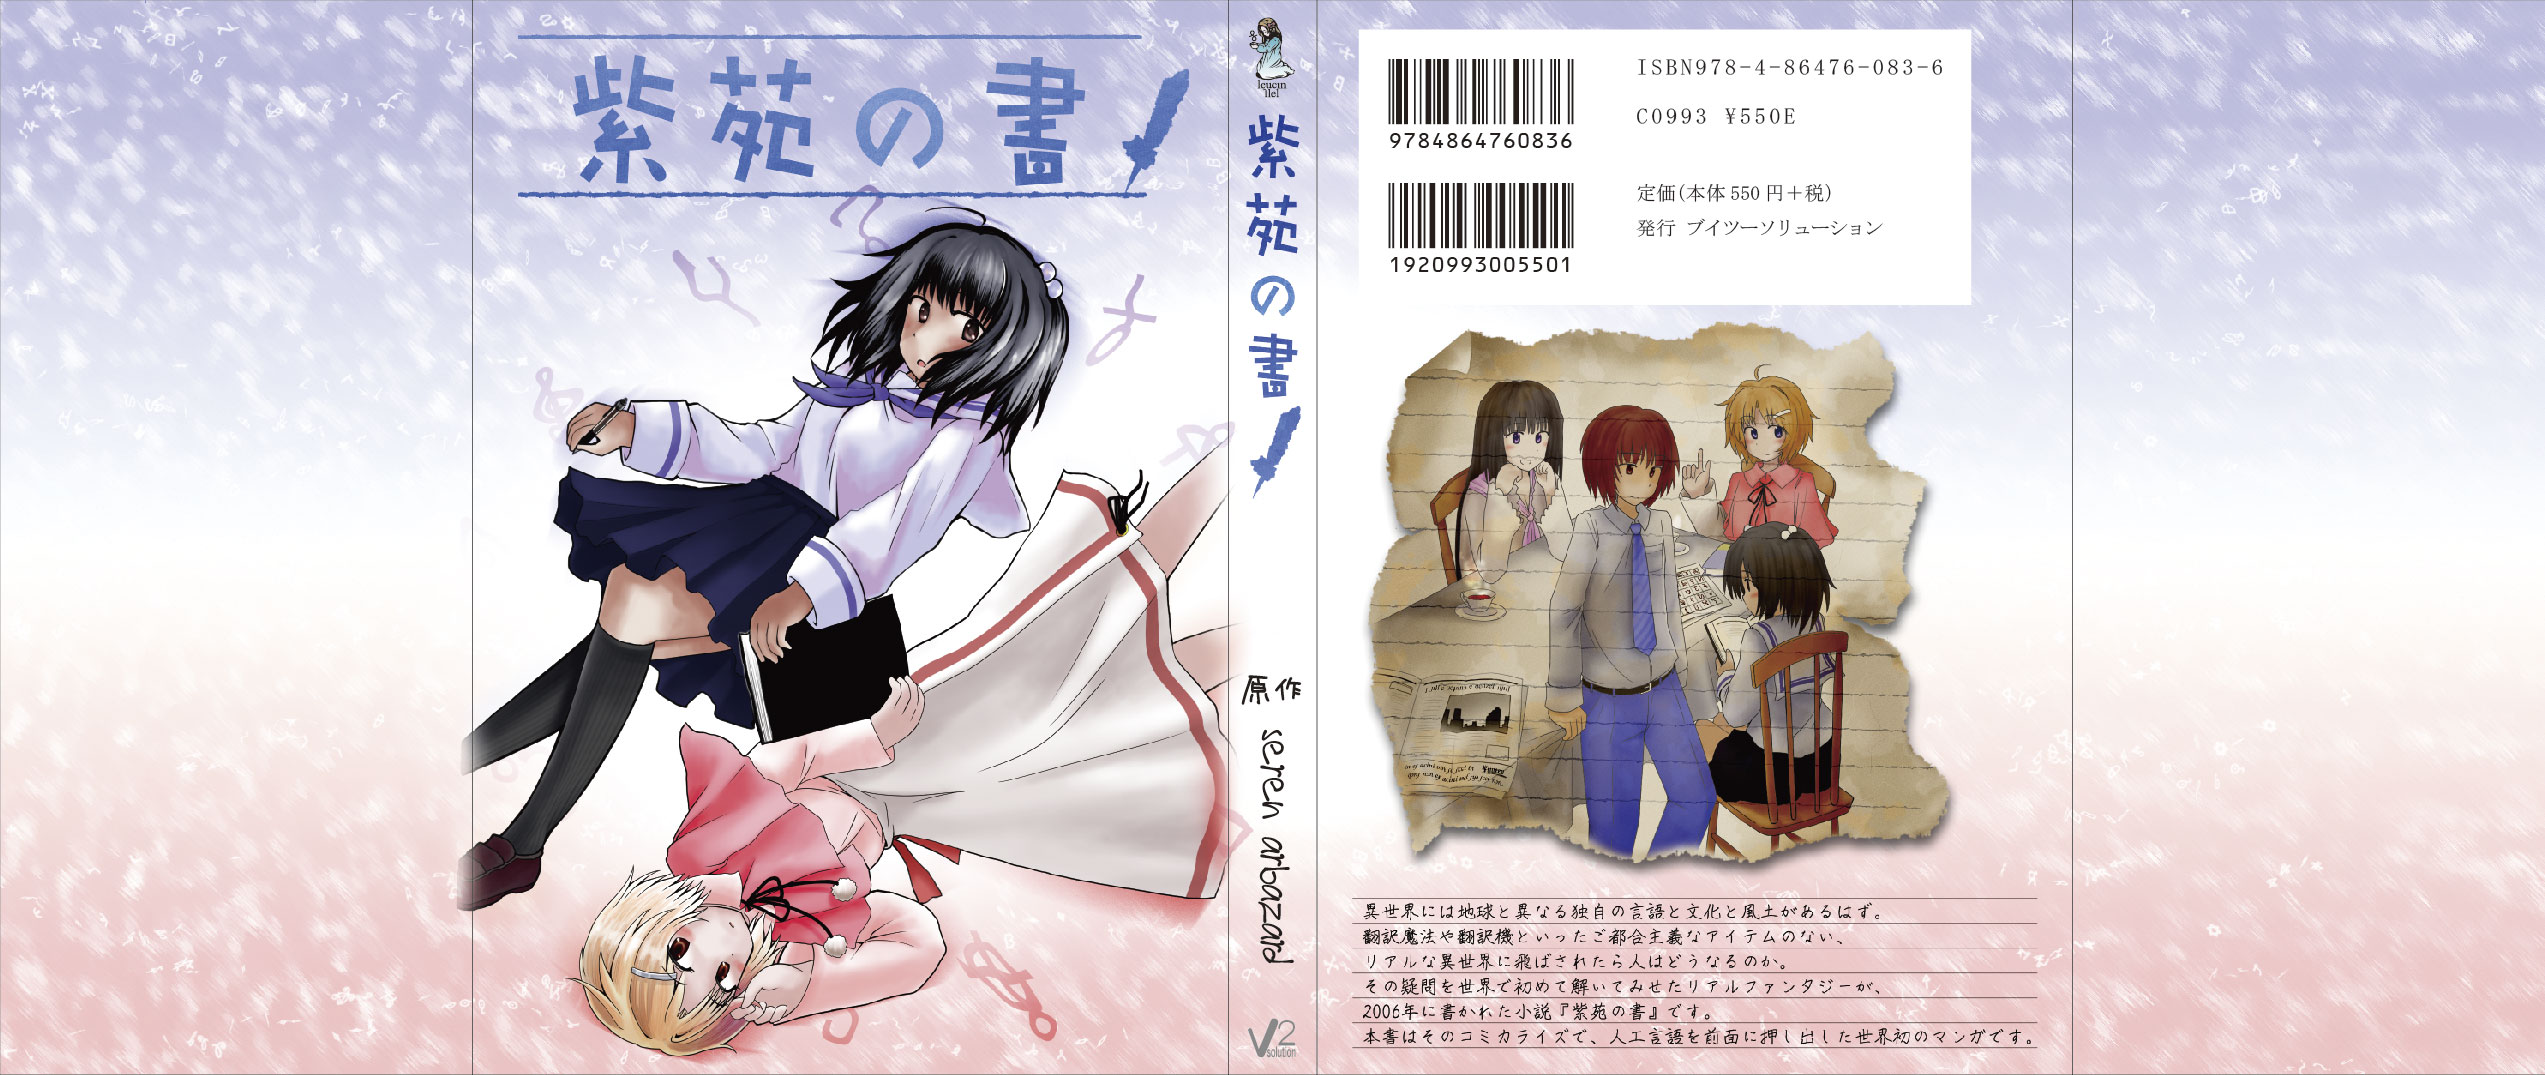
\includepdf[pages={1}]{cover.pdf} %曲线救国的思路,外界自建封面,然后调用
% \end{titlepage}